\documentclass[aspectratio=169, xcolor=table]{beamer}
\usetheme{TUDelft}

% ====================================================================
% ANIMATION TOGGLE
% ====================================================================
\newif\ifanimated
\animatedtrue
\ifdefined\staticmode
  \animatedfalse
\fi
\newcommand{\cpause}{\ifanimated\pause\fi}

% Import theme macros (includes TikZ libraries and semantic colors)
\usepackage{tikz}
\usetikzlibrary{positioning, shapes, arrows, shadows, fit, calc, decorations.pathreplacing}

% Semantic Colors - One meaning per color
\definecolor{irSparse}{HTML}{3498DB}   % Sparse/BM25: Blue
\definecolor{irDense}{HTML}{E67E22}    % Dense/Embeddings: Orange
\definecolor{irRerank}{HTML}{C0392B}   % Rerank/Cross-encoder: Red
\definecolor{irHybrid}{HTML}{2ECC71}   % Hybrid/Fusion: Green
\definecolor{irANN}{HTML}{9B59B6}      % ANN/Infra: Purple
\definecolor{irInfra}{HTML}{58595B}    % General Infra: Dark Gray
\definecolor{irMuted}{HTML}{D9D9D9}    % Faint Gray

% Base Styles - Consistent Diagram Grammar
\tikzset{
    irBoxBase/.style={
        rectangle, 
        draw, 
        rounded corners=2pt, 
        minimum height=0.8cm, 
        minimum width=2cm,
        font=\small\sffamily,
        align=center,
        drop shadow={opacity=0.15},
        inner sep=5pt
    },
    irDatabase/.style={
        cylinder, 
        draw, 
        shape border rotate=90, 
        aspect=0.25, 
        minimum height=1.2cm, 
        minimum width=1cm,
        fill=irMuted!20,
        draw=irInfra,
        font=\tiny\sffamily,
        align=center
    },
    % Semantic Variants
    sparse/.style={irBoxBase, fill=irSparse!10, draw=irSparse},
    dense/.style={irBoxBase, fill=irDense!10, draw=irDense},
    rerank/.style={irBoxBase, fill=irRerank!10, draw=irRerank},
    hybrid/.style={irBoxBase, fill=irHybrid!10, draw=irHybrid},
    ann/.style={irBoxBase, fill=irANN!10, draw=irANN},
    infra/.style={irBoxBase, fill=irInfra!10, draw=irInfra},
    % Legacy support / Utility
    muted/.style={irBoxBase, fill=irMuted!20, draw=irMuted!80!black, text=irMuted!50!black},
    ghost/.style={irBoxBase, fill=white, draw=irMuted!50, text=irMuted, dashed, drop shadow={opacity=0}},
    emph/.style={draw=irRerank, thick, drop shadow={shadow xshift=0mm, shadow yshift=0mm, fill=irRerank, opacity=0.3}},
    % Arrows
    irArrowBase/.style={->, thick, >=latex, draw=irInfra},
    irLabel/.style={
        font=\tiny\itshape, 
        text=irInfra, 
        align=center, 
        text width=2.5cm, 
        inner sep=3pt
    }
}


% =========================================================
% Stage Badge System
% =========================================================
% \irStage{StageName}
\newcommand{\irStage}[1]{%
    \begin{tikzpicture}[remember picture, overlay]
        \node[
            anchor=north east,
            fill=irInfra!10,
            text=irInfra,
            font=\tiny\bfseries,
            inner sep=3pt,
            rounded corners=1pt,
            yshift=-0.5cm,
            xshift=-0.5cm
        ] at (current page.north east) {#1};
    \end{tikzpicture}%
}

% =========================================================
% Math Highlighting
% =========================================================
% \mathhl[color]{content}
\newcommand{\mathhl}[2][irDense!30]{%
    \colorbox{#1}{$\displaystyle #2$}%
}

% =========================================================
% Math Vectors
% =========================================================
\newcommand{\vs}{\mathbf{s}}

% =========================================================
% Core Box Primitives
% =========================================================
% \IRBox[width]{id}{at}{title}{subtitle}{variant}
% Default width chosen for lecture slides; override when needed.
% \IRBox[width]{id}{at}{title}{subtitle}{variant}[extra options]
\DeclareDocumentCommand{\IRBox}{O{3.5cm} m m m m m O{}}{%
    \node[#6, text width=#1, #7] (#2) at #3 {%
        \textbf{#4}%
        \if\relax\detokenize{#5}\relax
        \else\\[-1mm]\scriptsize #5%
        \fi
    };%
}

% \IRWideBox{id}{at}{width}{title}{subtitle}{variant}
\newcommand{\IRWideBox}[6]{%
    \node[#6, text width=#3] (#1) at #2 {%
        \textbf{#4}%
        \if\relax\detokenize{#5}\relax
        \else\\[-1mm]\scriptsize #5%
        \fi
    };%
}

% =========================================================
% Arrow Primitives
% =========================================================
% Safe default: left-to-right flow
% \IRArrow{from}{to}{label}
\newcommand{\IRArrow}[3]{%
    \draw[irArrowBase] (#1.east) -- node[irArrowLabelAbove] {#3} (#2.west);%
}

% Explicit left-to-right
% \IRArrowLR{from}{to}{label}
\newcommand{\IRArrowLR}[3]{%
    \draw[irArrowBase] (#1.east) -- node[irArrowLabelAbove] {#3} (#2.west);%
}

% Explicit top-to-bottom
% \IRArrowTB{from}{to}{label}
\newcommand{\IRArrowTB}[3]{%
    \draw[irArrowBase] (#1.south) -- node[irArrowLabelRight] {#3} (#2.north);%
}

% Fully explicit anchor-to-anchor path
% \IRArrowPath{from anchor}{to anchor}{label}
% Example: \IRArrowPath{a.east}{b.north}{score}
\newcommand{\IRArrowPath}[3]{%
    \draw[irArrowBase] (#1) -- node[irArrowLabelAbove] {#3} (#2);%
}

% Orthogonal elbow path
% \IRArrowElbow{from anchor}{to anchor}{label}
% Example: \IRArrowElbow{a.east}{b.north}{feedback}
\newcommand{\IRArrowElbow}[3]{%
    \draw[irArrowBase] (#1) -| node[irArrowLabelBox] {#3} (#2);%
}

% Slanted arrow for special cases only
% \IRArrowSlanted{from anchor}{to anchor}{label}{pos}{width}
\newcommand{\IRArrowSlanted}[5]{%
    \draw[irArrowBase] (#1) -- node[above, sloped, irLabel, pos=#4, text width=#5, fill=white, inner sep=1pt] {#3} (#2);%
}

% =========================================================
% Accent Elements
% =========================================================
% \IRBadge{at}{text}
\newcommand{\IRBadge}[2]{%
    \node[
        draw=irAccent,
        fill=irAccent!20,
        rounded corners=1pt,
        font=\tiny\bfseries,
        inner sep=2pt
    ] at #1 {#2};%
}

% =========================================================
% Grouping
% =========================================================
% \IRGroup{fit nodes}{label}{variant}
% Example: \IRGroup{(a)(b)(c)}{First-stage retrieval}{muted}
\newcommand{\IRGroup}[3]{%
    \node[
        irGroupBase,
        #3,
        fit=#1
    ] (group) {};
    \node[
        anchor=north west,
        font=\tiny\bfseries,
        #3
    ] at ([xshift=2pt,yshift=-2pt] group.north west) {#2};%
}

% =========================================================
% Domain-Specific Shapes
% =========================================================
% \IRDocStack{id}{at}{label}
\newcommand{\IRDocStack}[3]{%
    \node[irDocStack] (#1) at #2 {#3};%
}

% \IRDatabase{id}{at}{label}
\newcommand{\IRDatabase}[3]{%
    \node[irDatabase] (#1) at #2 {#3};%
}

% =========================================================
% Layout Helpers
% =========================================================
% \IRPipelineTier{id}{at}{text}{label}{variant}
\newcommand{\IRPipelineTier}[5]{%
    \IRBox{#1}{#2}{#3}{}{#5}[]
    \node[anchor=west, irLabel, xshift=0.5cm] at (#1.east) {#4};%
}

% \IRTelescopeTier{id}{at}{width}{text}{variant}
\newcommand{\IRTelescopeTier}[5]{%
    \node[
        irTelescopeBase,
        #5,
        minimum width=#3
    ] (#1) at #2 {#4};%
}

% \IRStep{id}{at}{title}{subtitle}{variant}
% Creates a numbered step badge left of a box.
\newcommand{\IRStep}[5]{%
    \node[
        circle,
        draw=irAccent,
        fill=irAccent!20,
        font=\tiny\bfseries,
        inner sep=2pt
    ] (#1_num) at #2 {#1};
    \node[
        #5,
        text width=3.5cm,
        right=1.5cm of #1_num
    ] (#1) {%
        \textbf{#3}%
        \if\relax\detokenize{#4}\relax
        \else\\[-1mm]\scriptsize #4%
        \fi
    };
    \draw[irArrowBase, thin] (#1_num.east) -- (#1.west);%
}

\usetikzlibrary{arrows.meta}

% Additional packages for this lecture
\usepackage{booktabs}
\usepackage{listings}
\usepackage[most]{tcolorbox}
\usepackage{graphicx}

% Math definitions
\newcommand{\vq}{\mathbf{q}}
\newcommand{\vp}{\mathbf{p}}
\newcommand{\vd}{\mathbf{d}}
\newcommand{\vk}{\mathbf{k}}
\newcommand{\vv}{\mathbf{v}}
\newcommand{\vx}{\mathbf{x}}
\newcommand{\vw}{\mathbf{w}}
\newcommand{\vctx}{\mathbf{c}}
\DeclareMathOperator*{\argmax}{arg\,max}
\DeclareMathOperator*{\argmin}{arg\,min}

% Legacy color mappings for extracted TikZ
\colorlet{retrieval}{irSparse}
\colorlet{prompt}{irDense}
\colorlet{gen}{irRerank}
\colorlet{ops}{irANN}
\colorlet{warn}{irInfra}

% Title information
\title[QA and RAG]{Question Answering and Retrieval-Augmented Generation}
\subtitle{Lecture 7: From Extractive QA to Grounded Generation}
\author{Avishek Anand}
\institute{Information Retrieval}
\date{\today}

% Automatic Roadmap/Outline slide at the start of each section
\AtBeginSection[]
{
  \begin{frame}{Roadmap}
    \tableofcontents[currentsection]
  \end{frame}
}

\begin{document}

% =====================================================
\begin{frame}[plain]
\titlepage
\end{frame}
% =====================================================

\begin{frame}{Outline}
\tableofcontents
\end{frame}


% % ====================================================================
% % OUTLINE
% % ====================================================================
% \begin{frame}[shrink=45]{Outline (2 hours)}
% \small
% \begin{columns}[T]
% \begin{column}{0.48\textwidth}
% \begin{enumerate}
%   \item \textbf{Hook} (10 min): Why QA? What's hard?
%   \item \textbf{What is QA?} (15 min): taxonomy, metrics
%   \item \textbf{System Architectures} (15 min): retriever–reader, closed-book
%   \item \textbf{Hallucination Crisis} (15 min): when LLMs fail
%   \item \textbf{RAG 101} (10 min): the three-module system
%   \item \textbf{Original RAG model} (10 min): Lewis et al.\ 2020
% \end{enumerate}
% \end{column}
% \begin{column}{0.48\textwidth}
% \begin{enumerate}
%   \setcounter{enumi}{6}
%   \item \textbf{Retrieval Deep Dive} (15 min): chunking, late chunking, reformulation
%   \item \textbf{Beyond Single-Shot} (15 min): multi-step, DeRIVeR, dynamic search
%   \item \textbf{Engineering Reality} (10 min): LLM stacks
%   \item \textbf{Evaluation} (10 min): faithfulness, failure taxonomy
%   \item \textbf{Advanced Systems} (10 min): IR-CoT, Self-RAG
%   \item \textbf{System Design \& Wrapup} (10 min)
% \end{enumerate}
% \end{column}
% \end{columns}

% \vspace{0.4em}
% \begin{tcolorbox}[colback=gray!10,colframe=gray!40,title=Assumed known (not re-taught)]
% \footnotesize
% BM25/RM3/LMs, ANN (IVF+PQ/HNSW), cross-encoders, dense retrieval (DPR/ColBERT/ANCE), hybrid.
% \end{tcolorbox}
% \end{frame}

% ====================================================================
\section{Part 1 --- From Rankings to Direct Answer}
% ====================================================================

\begin{frame}[plain]
\sectionpage
\end{frame}

\begin{frame}{The Information Need}
% \irStage{MOTIVATION}
\textbf{We have always needed answers, not just documents.}

\vspace{0.8em}
\begin{itemize}
  \item \textbf{1990s Web Search}: returns \emph{documents} ranked by relevance
  \item \textbf{2011 IBM Watson}: returns a \emph{direct answer} (Jeopardy!)
  \item \textbf{2018 BERT}: reads a passage and \emph{extracts} an answer span
  \item \textbf{2020 GPT-3}: \emph{generates} answers from parametric memory
  \item \textbf{2020 RAG}: \emph{retrieves then generates}---evidence-grounded
\end{itemize}

\vspace{0.3em}
\begin{block}{The Core Tension}
\small
Retrieval gives us \textbf{evidence} but cannot reason. Generation gives us \textbf{fluency} but can fabricate. \textbf{QA} needs both.
\end{block}
\end{frame}

\begin{frame}[shrink=25]{What Does a QA System Do?}
\textbf{Input: natural language question $q$. \quad Output: direct answer $a$.}

\vspace{0.8em}
\begin{columns}[T]
\begin{column}{0.55\textwidth}
\large
\begin{block}{Contrast with document retrieval}
\begin{itemize}
  \item Document IR: returns a \emph{ranked list} of passages
  \item QA: returns a \emph{single concise answer}
  \item Same retrieval stack---different answer contract
\end{itemize}
\end{block}
\cpause
\begin{block}{Why harder?}
\begin{itemize}
  \item Questions are short, ambiguous, or multi-part
  \item Evidence may be split across multiple passages
  \item Answer must be correct---not just relevant
\end{itemize}
\end{block}
\end{column}
\begin{column}{0.42\textwidth}
\begin{center}
\resizebox{0.9\textwidth}{!}{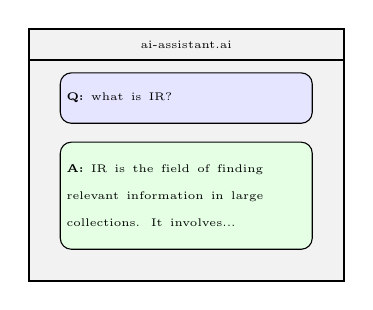
\begin{tikzpicture}[scale=0.8, every node/.style={transform shape}]
    % Mock chat
    \draw[thick, fill=gray!10] (0,0) rectangle (5,4);
    \draw[thick] (0,3.5) -- (5,3.5);
    \node at (2.5, 3.75) {\tiny ai-assistant.ai};
    
    % Chat bubble
    \draw[fill=blue!10, rounded corners] (0.5, 2.5) rectangle (4.5, 3.3);
    \node[text width=3.8cm] at (2.5, 2.9) {\tiny \textbf{Q:} what is IR?};
    
    % Answer bubble
    \draw[fill=green!10, rounded corners] (0.5, 0.5) rectangle (4.5, 2.2);
    \node[text width=3.8cm] at (2.5, 1.35) {\tiny \textbf{A:} IR is the field of finding relevant information in large collections. It involves...};
\end{tikzpicture}
}
\end{center}
\end{column}
\end{columns}
\end{frame}


\begin{frame}[shrink=5]{What is Closed-Book QA ?}
% \irStage{ARCHITECTURE}
\cpause

\textbf{Answer everything from the model's parametric memory.}

\begin{center}
\fbox{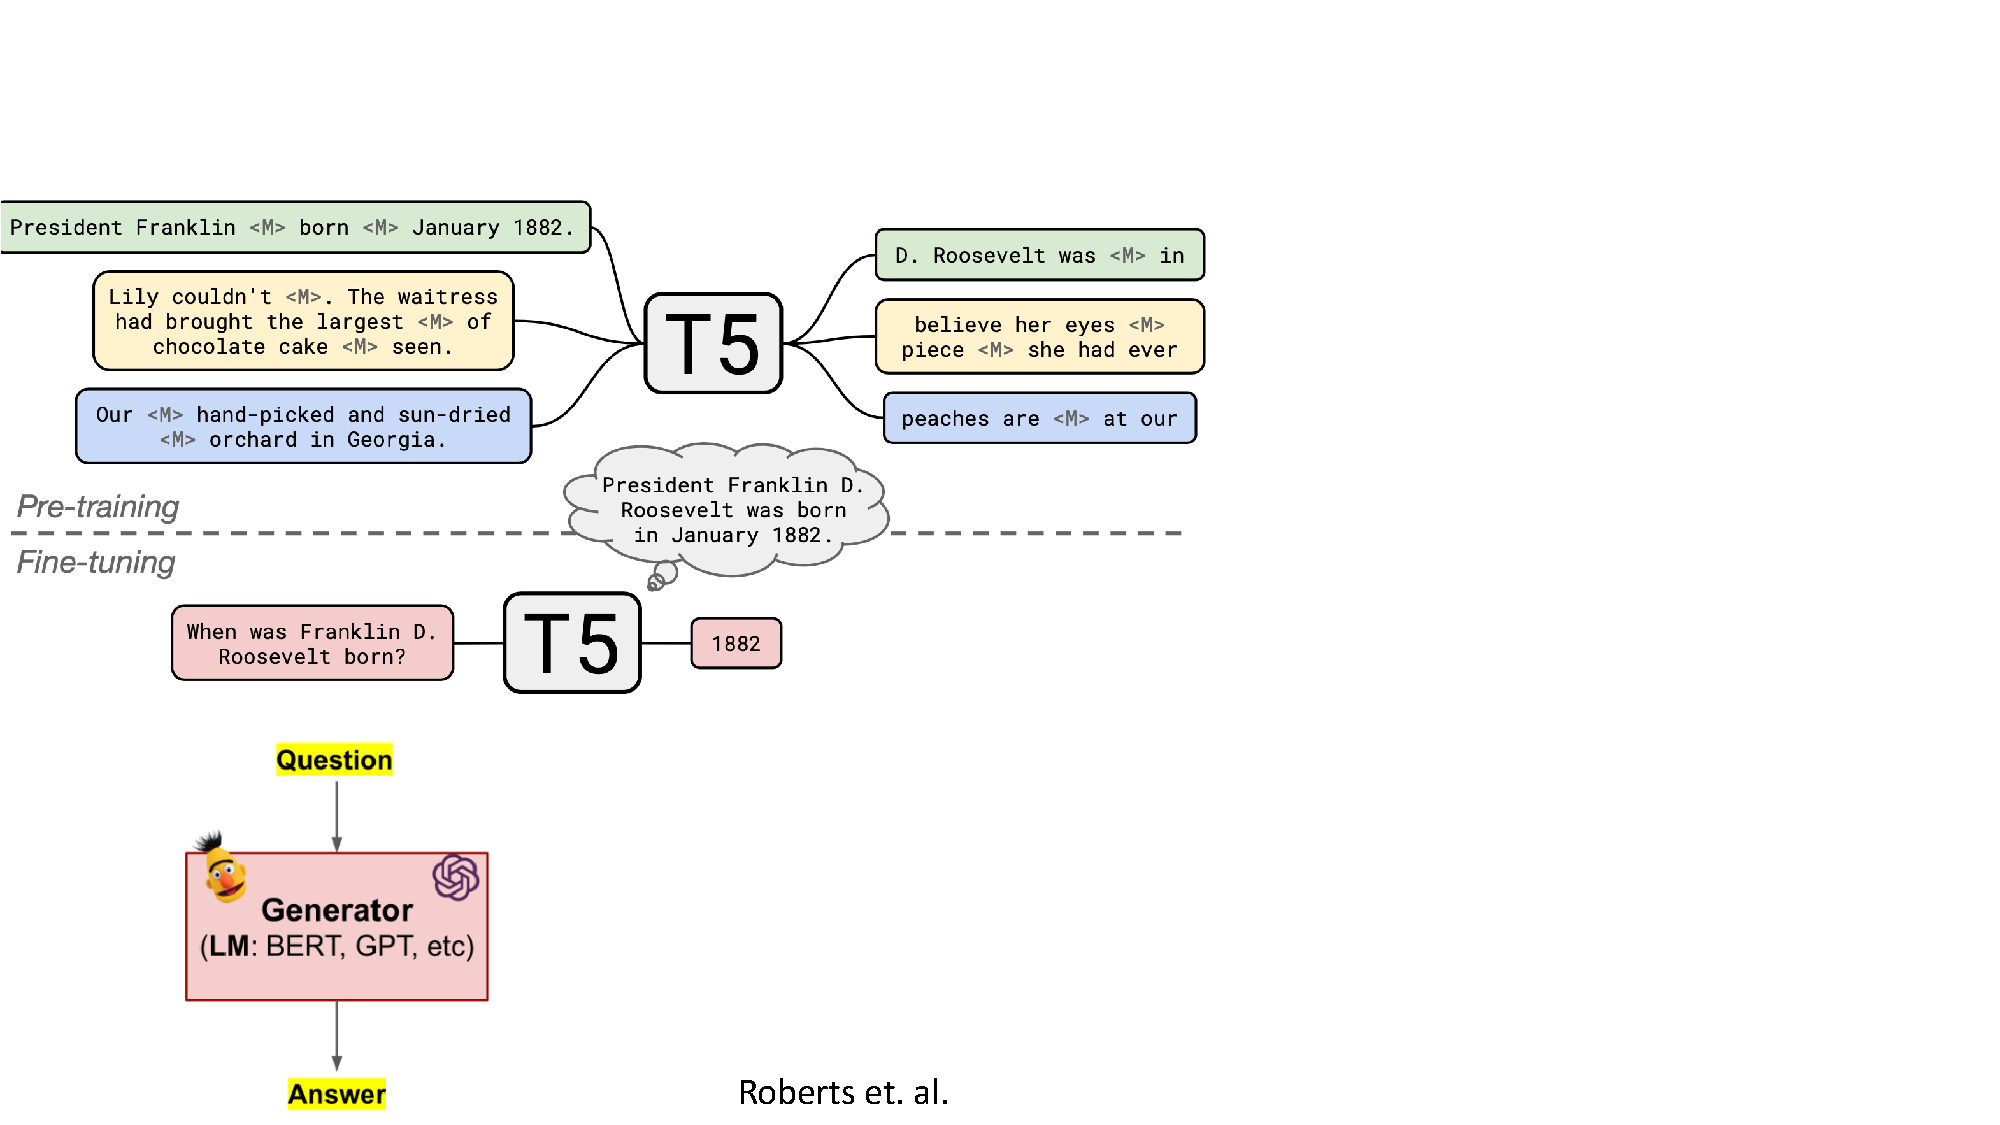
\includegraphics[height=0.72\textheight, keepaspectratio]{figures/closedbook-qa.pdf}}
\end{center}
\end{frame}

\begin{frame}[shrink=20]{Why Closed-Book QA Falls Short}
% \irStage{LIMITATIONS}
\textbf{LLMs can answer many questions without retrieval---but fail in predictable ways.}

\cpause

\vspace{0.7em}
\begin{columns}[T]
\begin{column}{0.52\textwidth}
\begin{itemize}
  \item \textbf{Knowledge cutoff}: no access to post-training facts
  \item \textbf{Long-tail failure}: rare entities poorly represented in weights
  \item \textbf{No evidence}: cannot cite sources; auditing is impossible
  \item \textbf{Hallucination}: confident generation of plausible but false content
\end{itemize}
\end{column}
\cpause
\begin{column}{0.44\textwidth}
\begin{block}{The Scale Paradox}
\small
Larger models hallucinate \emph{more confidently}---not less.\\[0.4em]
Scale alone does not solve factual grounding.
\end{block}
\end{column}
\end{columns}

\vspace{0.5em}
\cpause
\begin{block}{Consequence}
For knowledge-intensive tasks in production, closed-book QA is not deployable without a grounding mechanism.
\end{block}
\end{frame}

\begin{frame}[shrink=18]{What Is Hallucination?}
% \irStage{FAILURE MODE}
\textbf{Hallucination: factually incorrect content presented with confidence.}

\cpause

\vspace{0.7em}
\begin{block}{Two types}
\begin{itemize}
  \item \textbf{Intrinsic}: contradicts the given context or source
  \item \textbf{Extrinsic}: asserts facts absent from any source (pure fabrication)
\end{itemize}
\end{block}

\cpause
\begin{block}{Why it's not a bug}
\begin{itemize}
  \item LLMs are trained to maximize token likelihood, not truth
  \item The model has no external factuality check at inference
  \item Fluent generation $\neq$ faithful generation
\end{itemize}
\end{block}

\cpause
\textbf{Danger} \\
\begin{itemize}
  \item Hallucinations look identical to correct answers in output format.
  \item Users cannot distinguish them without external verification.
\end{itemize}
\end{frame}

\begin{frame}{Hallucinations in the Wild}
% \irStage{EXAMPLES}
\cpause
\begin{center}
\fbox{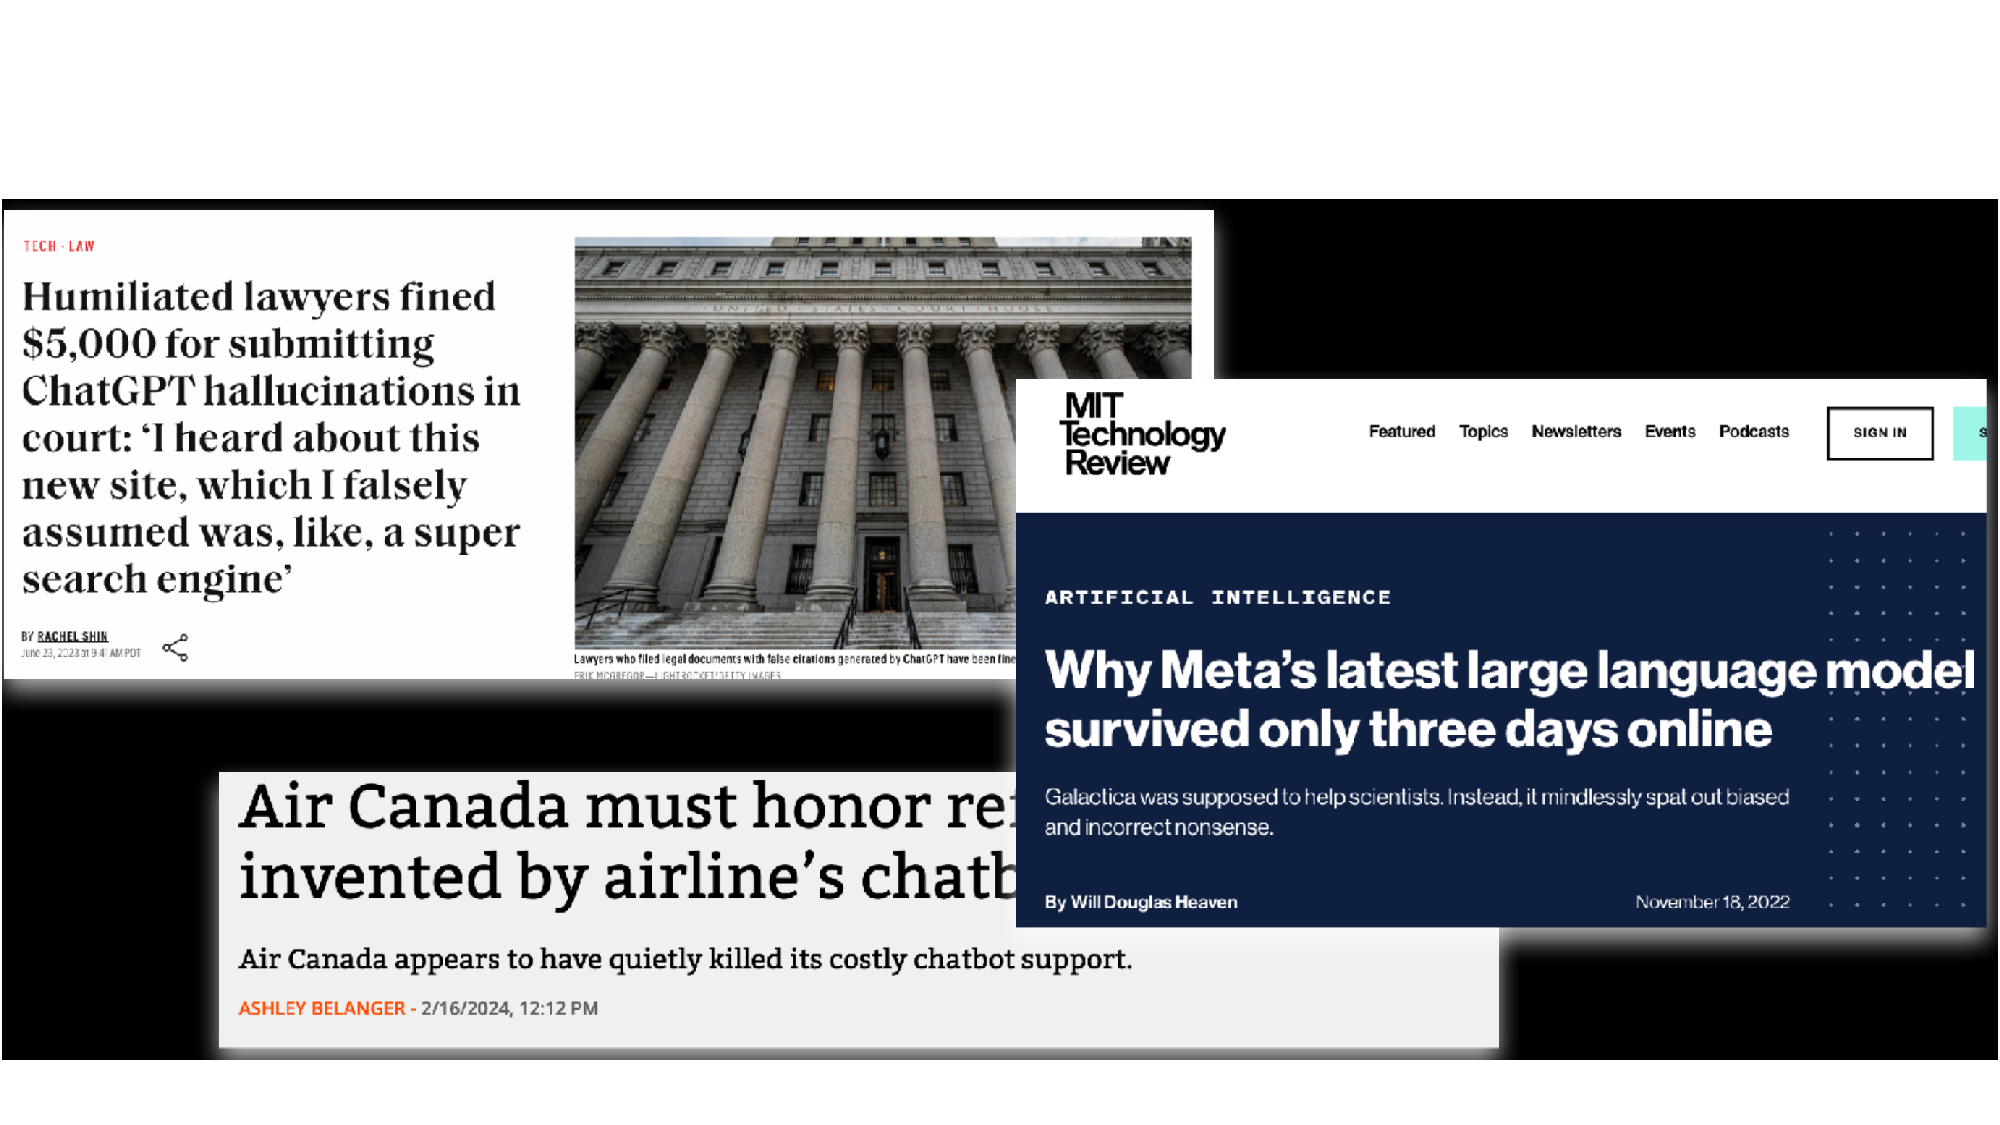
\includegraphics[width=0.82\textwidth]{figures/hallucination-many.pdf}}
\end{center}
\end{frame}

\begin{frame}{High-Stakes Hallucination}
% \irStage{CASE STUDY}
\begin{center}
\fbox{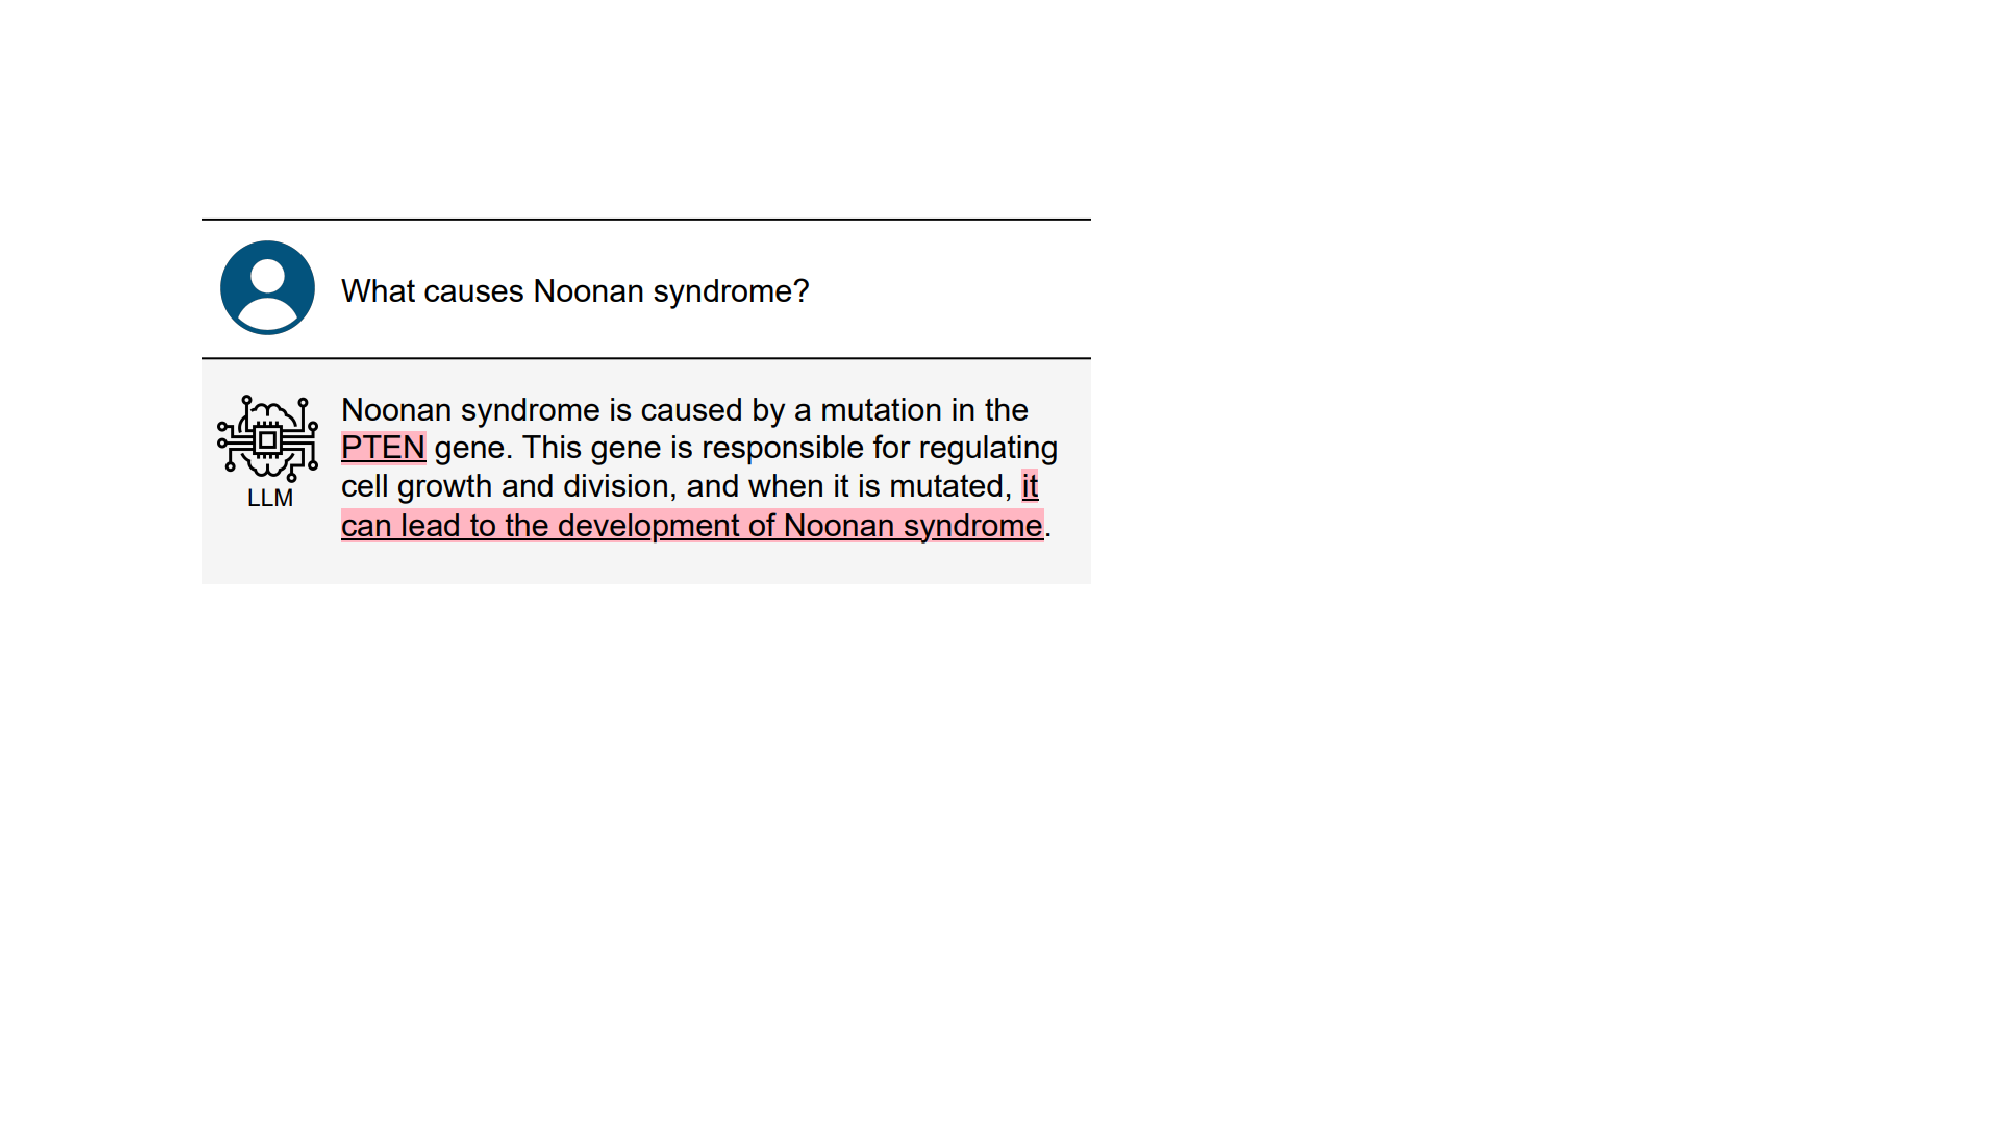
\includegraphics[width=0.82\textwidth]{figures/hallucination-noonan.pdf}}
\end{center}
\end{frame}

\begin{frame}{Why Do LLMs Hallucinate?}
% \irStage{ROOT CAUSE}
\textbf{Multiple independent failure modes compound at inference time.}

\vspace{0.7em}
\begin{columns}[T]
\begin{column}{0.52\textwidth}
\begin{enumerate}
  \item \textbf{Training data noise}: web text contains errors, contradictions
  \item \textbf{Distributional gaps}: rare or unseen entity combinations
  \item \textbf{Autoregressive bias}: each token conditions on previous tokens only; no global fact check
  \item \textbf{RLHF side-effects}: helpfulness reward may override accuracy
\end{enumerate}
\end{column}
\begin{column}{0.44\textwidth}
\begin{block}{The Core Problem}
\small
There is no ``ground truth'' signal during autoregressive generation.\\[0.3em]
The model generates the \emph{most likely} continuation, not the \emph{most true} one.
\end{block}
\end{column}
\end{columns}
\end{frame}

\begin{frame}[shrink=10]{RAG as the Answer to Hallucination}
% \irStage{SOLUTION}
\textbf{Grounding generation in retrieved evidence constrains what the model can say.}

\vspace{0.7em}
\begin{itemize}
  \item Retrieved evidence is \textbf{explicit} and \textbf{checkable}
  \item Model is prompted to cite evidence: \emph{``use only what is in the passages''}
  \item Claims without evidence support can be automatically flagged
  \item Index can be updated without retraining the LLM
\end{itemize}

\vspace{0.6em}
\cpause
\begin{block}{Retrieval defines the reasoning substrate}
If evidence is not retrieved, it cannot be used. But if it \emph{is} retrieved, attribution is possible.
\end{block}
\end{frame}

\begin{frame}[shrink=5]{QA as a Task Family}
% \irStage{TAXONOMY}
\textbf{``QA'' is an umbrella for many different tasks with different assumptions.}

\vspace{0.5em}
\begin{table}
\centering
\resizebox{0.95\textwidth}{!}{
\begin{tabular}{l l l l}
\toprule
\textbf{Type} & \textbf{Input} & \textbf{Output} & \textbf{Benchmark} \\
\midrule
Extractive      & Question + passage  & Span in passage       & SQuAD, NewsQA \\
\cpause Abstractive     & Question + passage  & Generated string      & NarrativeQA, CoQA \\
\cpause Open-Domain     & Question only       & Answer (from corpus)  & Natural Questions, TriviaQA \\
\cpause Knowledge-Base  & Question + KG       & Entity/relation       & WebQuestions, LC-QuAD \\
\cpause Conversational  & Multi-turn history  & Answer in context     & QuAC, DoQA \\
\bottomrule
\end{tabular}
}
\end{table}

\vspace{0.4em}
\cpause
\begin{block}{This lecture's focus}
\textbf{Open-domain QA}: no passage given---the system must retrieve it.
RAG is the dominant approach for open-domain QA at scale.
\end{block}
\end{frame}

\begin{frame}[shrink=20]{Open-Domain QA: The Setup}
% \irStage{FORMALIZATION}
\textbf{The problem: find an answer in a large corpus without knowing where to look.}

\vspace{0.8em}
\textbf{Formal setup:}
\begin{itemize}
  \item Given: question $q$ and corpus $\mathcal{C} = \{d_1, d_2, \ldots, d_N\}$
  \item Goal: produce answer $a$
  \item Step 1 (Retrieve): $\mathcal{R}_k(q) \subset \mathcal{C}$, top-$k$ passages
  \item Step 2 (Read/Generate): $a = f(q,\, \mathcal{R}_k(q))$
\end{itemize}


\vspace{0.5em}
\begin{block}{Key Insight}
\small
The retrieval step is the bottleneck. If $e^\star \notin \mathcal{R}_k(q)$, then $P(\text{correct}) \approx 0$.
\textbf{All QA quality is bounded by retrieval quality.}
\end{block}
\end{frame}

\begin{frame}[shrink=10]{How do we evaluate the Answers ?}
% \irStage{EVALUATION}
\cpause
\textbf{The two standard metrics for extractive and short-answer QA.}

\vspace{0.7em}
\begin{block}{Exact Match (EM)}
Binary: normalized prediction = normalized gold?\\[0.3em]
\footnotesize Normalization: lowercase, strip articles \& punctuation, collapse whitespace.
\end{block}

\vspace{0.4em}
\begin{block}{Token F1}
Token-level overlap between prediction and gold:
\[ F_1 = \frac{2 \cdot P \cdot R}{P + R} \]
\footnotesize $P$: matched / \#predicted, \quad $R$: matched / \#gold
\end{block}
\end{frame}

% \begin{frame}[shrink=10]{Evaluation: Limitations}
% % \irStage{EVALUATION}
% \textbf{EM and F1 have limitations when dealing with generated or abstractive answers.}
% \cpause
% \begin{block}{Running example}
% Question: \emph{Who won Super Bowl 50?}; Gold answer: \texttt{Denver Broncos}

% \begin{tabular}{l c c}
% Prediction & EM & F1 \\
% \midrule
% \texttt{Denver Broncos} & 1 & 1.0 \\
% \texttt{The Denver Broncos} & 0 & 0.80 \\
% \texttt{Broncos} & 0 & 0.67 \\
% \end{tabular}
% \end{block}

% \vspace{0.7em}
% \begin{block}{Limitation}
% \large
% EM/F1 are sensitive to valid paraphrases:\\[0.5em]
% ``automobile'' $\neq$ ``car'' by EM\\
% but semantically equivalent.\\[0.8em]
% Works well for span extraction; breaks for abstractive answers.
% \end{block}
% \end{frame}



%% New code

% \begin{frame}[shrink=10]{Evaluation: Exact Match and Token F1}
% \irStage{EVALUATION}
% \textbf{Standard metrics for extractive QA.}

% \vspace{0.5em}
% \begin{block}{Exact Match (EM)}
% Binary, all-or-nothing:
% \[
% \mathrm{EM}(a,\hat a)=
% \begin{cases}
% 1 & \text{if prediction exactly matches a gold answer}\\
% 0 & \text{otherwise}
% \end{cases}
% \]
% \footnotesize Strict metric: even a small surface difference gives 0.
% \end{block}

% \vspace{0.3em}
% \begin{block}{Token F1}
% Soft overlap between predicted and gold answer tokens:
% \[
% F_1 = \frac{2PR}{P+R}
% \qquad
% P = \frac{|\text{pred} \cap \text{gold}|}{|\text{pred}|},
% \quad
% R = \frac{|\text{pred} \cap \text{gold}|}{|\text{gold}|}
% \]
% \footnotesize Rewards partial matches at token level.
% \end{block}

% \vspace{0.3em}
% \begin{block}{Running example}
% Question: \emph{Who won Super Bowl 50?}; Gold answer: \texttt{Denver Broncos}

% \begin{tabular}{l c c}
% Prediction & EM & F1 \\
% \midrule
% \texttt{Denver Broncos} & 1 & 1.0 \\
% \texttt{The Denver Broncos} & 0 & 0.80 \\
% \texttt{Broncos} & 0 & 0.67 \\
% \end{tabular}
% \end{block}
% \end{frame}


\begin{frame}[shrink=10]{Evaluation: When EM and F1 Make Sense}
% \irStage{EVALUATION}
\cpause
\textbf{They are best suited for span-based answers.}

\vspace{0.6em}
\begin{columns}[T]
\begin{column}{0.48\textwidth}
\begin{block}{When EM makes sense}
\begin{itemize}
  \item Extractive QA
  \item Short factoid answers
  \item Benchmarking exact span prediction
\end{itemize}

\vspace{0.3em}
\textbf{Example:}\\
Gold: \texttt{Paris}\\
Prediction: \texttt{Paris}\\
\[
\mathrm{EM}=1,\quad F_1=1
\]
\end{block}
\end{column}

\begin{column}{0.48\textwidth}
\begin{block}{When F1 makes sense}
\begin{itemize}
  \item Extractive QA with near misses
  \item Boundary errors in span extraction
  \item Partially correct short answers
\end{itemize}

\vspace{0.3em}
\textbf{Example:}\\
Gold: \texttt{Denver Broncos}\\
Prediction: \texttt{The Denver Broncos}\\
\[
\mathrm{EM}=0,\quad F_1=0.80
\]
\end{block}
\end{column}
\end{columns}

\vspace{0.6em}
\begin{block}{Takeaway}
EM is useful when you care about \textbf{exact answer strings}.  
F1 is useful when you care about \textbf{partial lexical overlap}.
\end{block}
\end{frame}


\begin{frame}[shrink=10]{Evaluation: Limitations of EM and F1}
\irStage{EVALUATION}
\cpause
\textbf{String overlap is not the same as semantic equivalence.}

\vspace{0.7em}
\begin{block}{Failure case for EM/F1}
Question: \emph{What is another word for automobile?}

\vspace{0.3em}
Gold answer: \texttt{car} \\
Prediction: \texttt{automobile}

\vspace{0.4em}
\[
\mathrm{EM}=0,\qquad F_1=0
\]

\vspace{0.4em}
\large
But the prediction is semantically correct.
\end{block}

\vspace{0.5em}
\cpause
\begin{block}{Why this matters}
\begin{itemize}
  \item Valid paraphrases are penalized
  \item Generated answers may use different wording
  \item EM/F1 work well for extractive QA, but break for abstractive QA
\end{itemize}
\end{block}
\end{frame}


\begin{frame}[shrink=10]{Evaluation: BERTScore Intuition}
\irStage{EVALUATION}
\textbf{Contextual token alignment for semantic similarity.}

\begin{center}
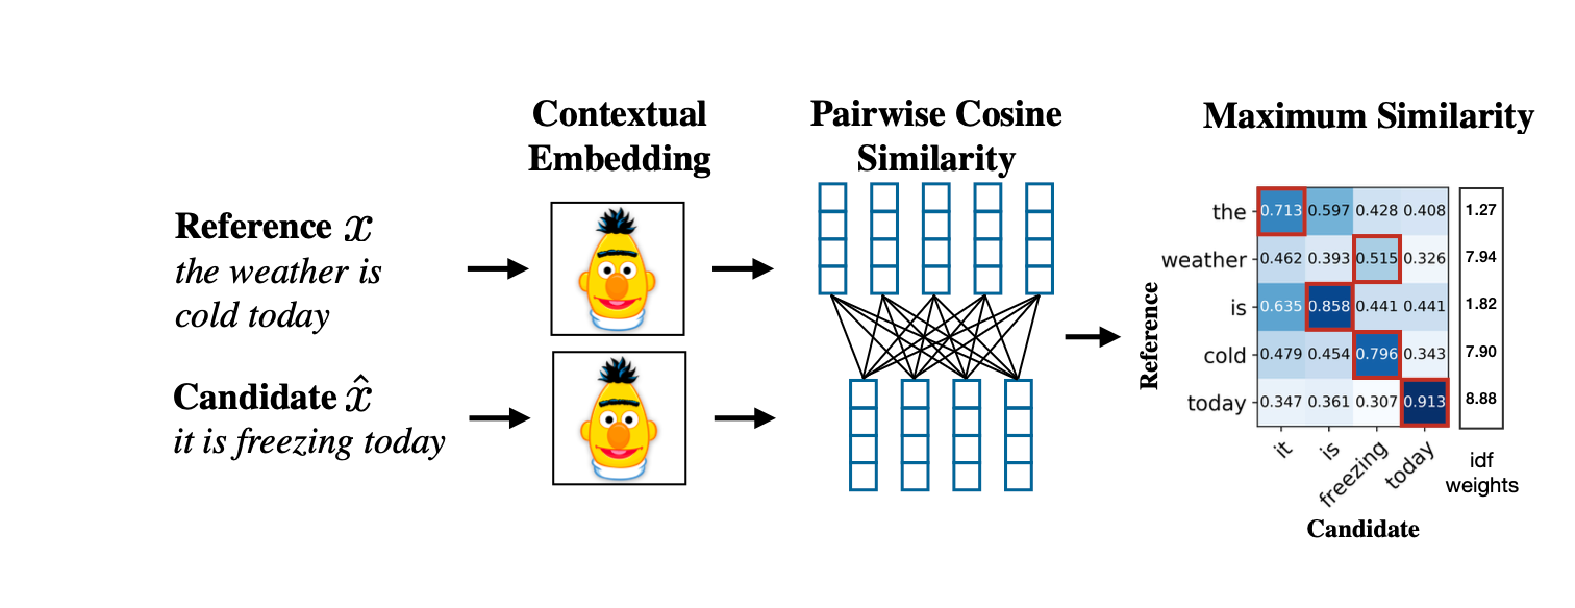
\includegraphics[width=0.8\textwidth]{figures/bertscore.pdf}
\end{center}

\vspace{-0.5em}
\begin{block}{Core Formulae}
\centering
\small
$R_{\text{BERT}} = \frac{1}{|x|} \sum_{x_i \in x} \max_{\hat{x}_j \in \hat{x}} \mathbf{x}_i^\top \mathbf{\hat{x}}_j$ \qquad
$P_{\text{BERT}} = \frac{1}{|\hat{x}|} \sum_{\hat{x}_j \in \hat{x}} \max_{x_i \in x} \mathbf{x}_i^\top \mathbf{\hat{x}}_j$ \\[0.5em]
$F_{\text{BERT}} = 2 \frac{P_{\text{BERT}} \cdot R_{\text{BERT}}}{P_{\text{BERT}} + R_{\text{BERT}}}$
\end{block}
\end{frame}


\begin{frame}[shrink=10]{Evaluation: BERTScore Details}
\irStage{EVALUATION}
\textbf{How BERTScore works (Zhang et al., 2020).}

\vspace{0.7em}
\begin{itemize}
  \item \textbf{Embeddings}: Represent reference $x$ and candidate $\hat{x}$ tokens with contextual embeddings (BERT, RoBERTa, etc.)
  \item \textbf{Matching}: Greedily match each token in $x$ to the most similar token in $\hat{x}$ using cosine similarity
  \item \textbf{Weighting}: Optional IDF weighting can emphasize more informative tokens
  \item \textbf{Robustness}: Handles paraphrases and synonyms where string-based metrics fail
\end{itemize}
\end{frame}


\begin{frame}[shrink=10]{Evaluation: When BERTScore Makes Sense}
\irStage{EVALUATION}
\textbf{BERTScore is useful when wording differs but meaning is preserved.}

\vspace{0.7em}
\begin{block}{Concrete running example}
Question: \emph{How is the weather today?}

\vspace{0.3em}
Reference answer: \texttt{the weather is cold today} \\
Candidate answer: \texttt{it is freezing today}

\vspace{0.5em}
\begin{itemize}
  \item EM = 0
  \item Token F1 is low or 0, depending on tokenization/overlap
  \item BERTScore is high because \texttt{cold} and \texttt{freezing} are semantically similar
\end{itemize}
\end{block}

\vspace{0.5em}
\cpause
\begin{block}{When to use what}
\begin{tabular}{l l}
Task type & Metric \\
\midrule
Extractive span QA & EM + F1 \\
Near-miss span prediction & F1 \\
Abstractive / paraphrastic QA & BERTScore \\
RAG systems & + Faithfulness / Attribution \\
\end{tabular}
\end{block}
\end{frame}


\begin{frame}[shrink=10]{Task-Level vs.\ System-Level Evaluation}
\irStage{EVALUATION}
\textbf{Answer quality is necessary, but not sufficient for QA systems.}

\vspace{0.7em}
\begin{columns}[T]
\begin{column}{0.48\textwidth}
\begin{block}{Task-Level}
EM, F1, ROUGE, BERTScore

\footnotesize
Question: \emph{Is the answer text correct or similar to gold?}
\end{block}
\end{column}
\begin{column}{0.48\textwidth}
\begin{block}{System-Level}
Faithfulness, Attribution, Hallucination rate

\footnotesize
Question: \emph{Is the answer actually grounded in retrieved evidence?}
\end{block}
\end{column}
\end{columns}

\vspace{0.7em}
\cpause
\begin{block}{Key insight}
A system can produce a plausible answer and score well on overlap-based metrics,
while still hallucinating unsupported claims.
\end{block}
\end{frame}
 

% ====================================================================
\section{Part 2 --- RAG 101}
% ====================================================================


\begin{frame}[plain]
\sectionpage
\end{frame}


\begin{frame}[shrink=15]{The Retriever--Reader Paradigm}
% \irStage{HISTORY}
\textbf{DrQA (Chen et al., 2017): the first large-scale open-domain neural QA system.}

\begin{itemize}
  \item \textbf{Stage 1 — Document Retriever}: TF-IDF over Wikipedia bigrams
  \item \textbf{Stage 2 — Document Reader}: BiLSTM (later BERT) extracts answer span
  \item Corpus: Wikipedia dump ($\approx$5M articles)
  \item Key insight: Wikipedia is a sufficiently comprehensive open-domain corpus
\end{itemize}

\begin{block}{Two-stage contract}
\footnotesize
Retriever maximizes passage recall. Reader maximizes span precision given top-$k$ passages.
\end{block}

\end{frame}

\begin{frame}{Retriever--Reader Architecture}
% \irStage{ARCHITECTURE}
\begin{center}
\fbox{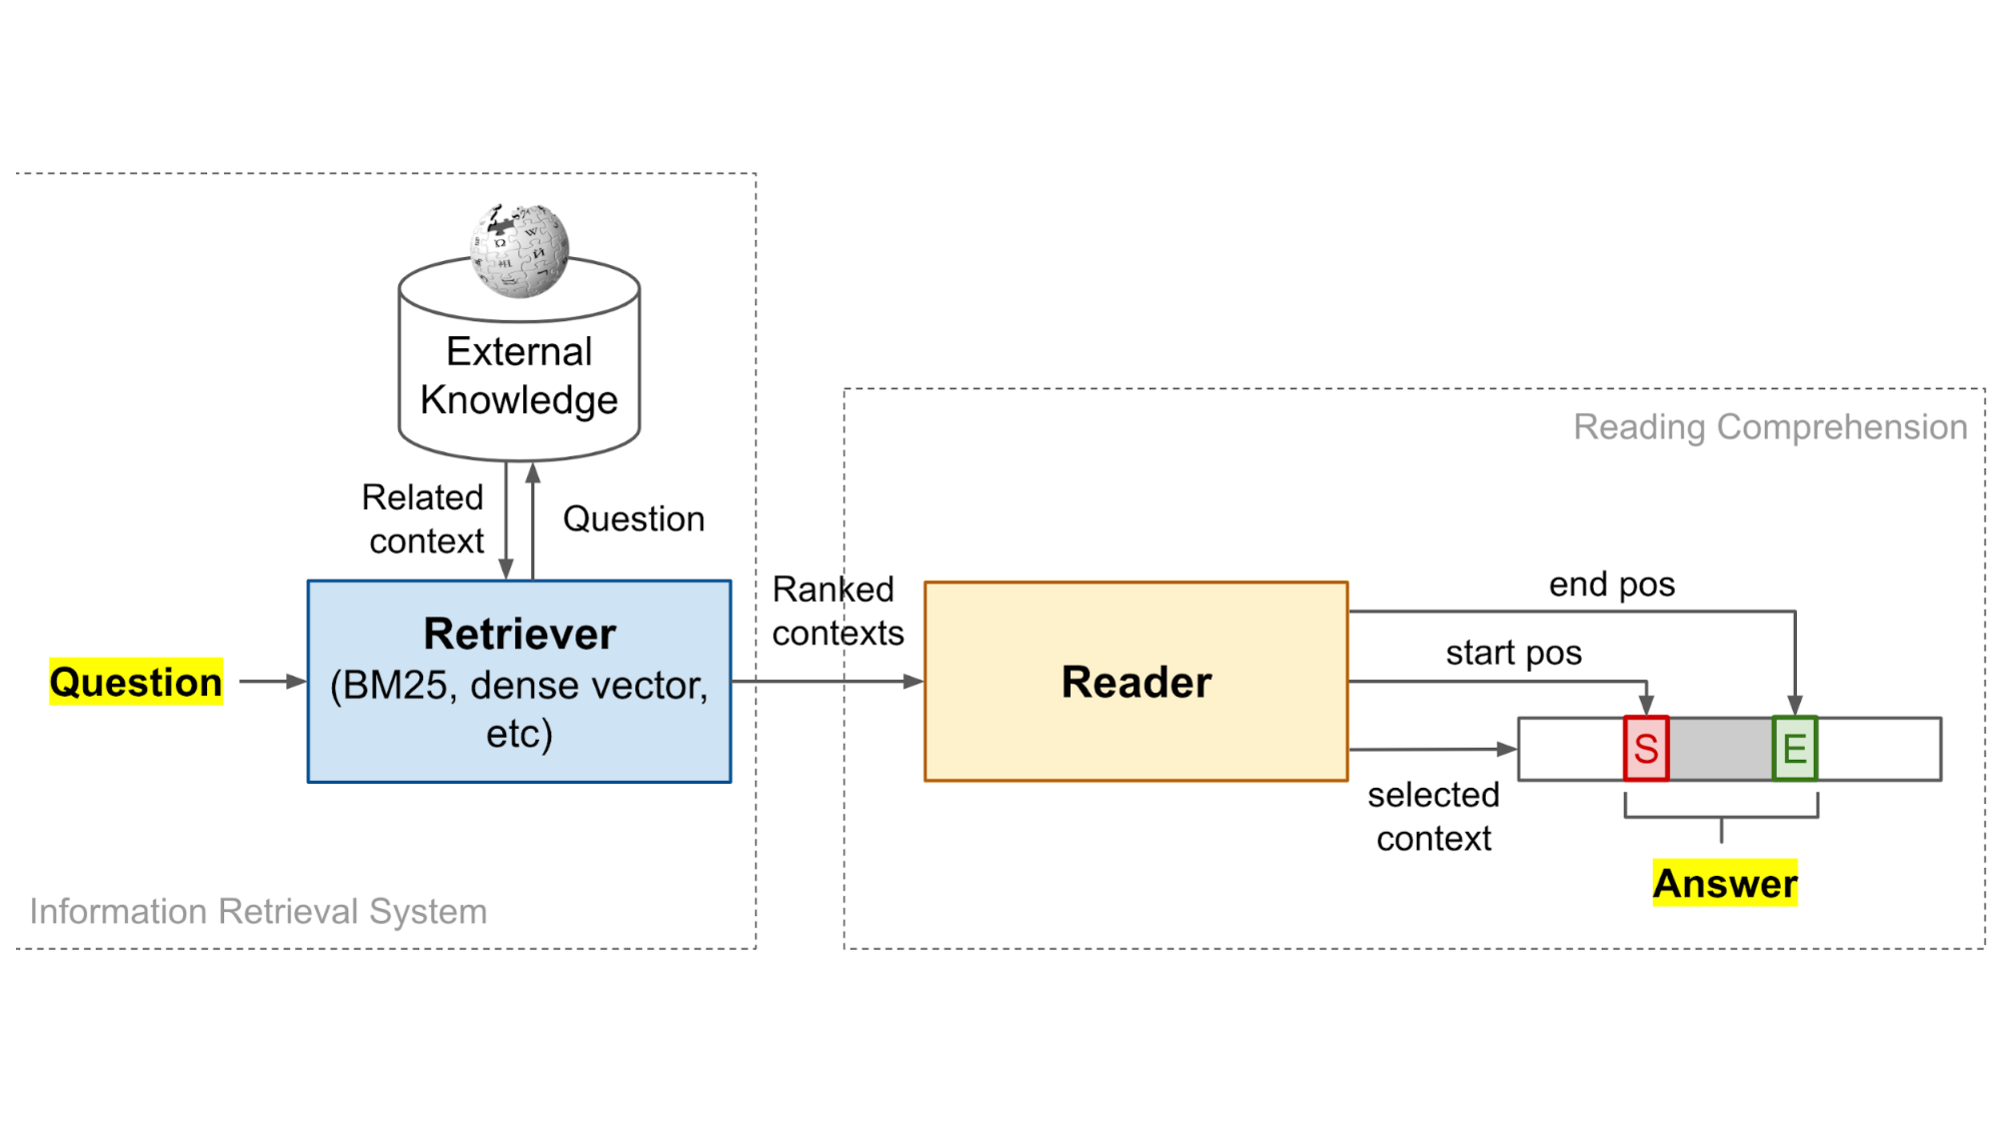
\includegraphics[width=0.82\textwidth]{figures/retriever-reader-qa.pdf}}
\end{center}
\end{frame}


\begin{frame}{Parametric vs. non-parametric knowledge}
% \irStage{MOTIVATION}
\cpause
\textbf{Parametric vs.\ non-parametric knowledge---both are incomplete alone.}

\vspace{0.8em}
\begin{columns}[T]
\begin{column}{0.48\textwidth}
\begin{block}{Parametric (LLMs)}
\begin{itemize}
  \item Knowledge baked into weights during training
  \item Fast at inference, no index required
  \item \textbf{Fails}: stale data, rare facts, confident errors
\end{itemize}
\end{block}
\end{column}
\begin{column}{0.48\textwidth}
\begin{block}{Non-parametric (Retrieval)}
\begin{itemize}
  \item Knowledge in an external, updatable index
  \item Evidence is explicit, citable, fresh
  \item \textbf{Fails}: retrieval errors propagate; cannot reason alone
\end{itemize}
\end{block}
\end{column}
\end{columns}

\vspace{0.7em}
\cpause
\begin{block}{RAG = Parametric + Non-Parametric}
Use retrieval to supply grounded evidence; use the LLM to reason over it.
\end{block}
\end{frame}

\begin{frame}{A General RAG Architecture}
% \irStage{ARCHITECTURE}
\begin{center}
\fbox{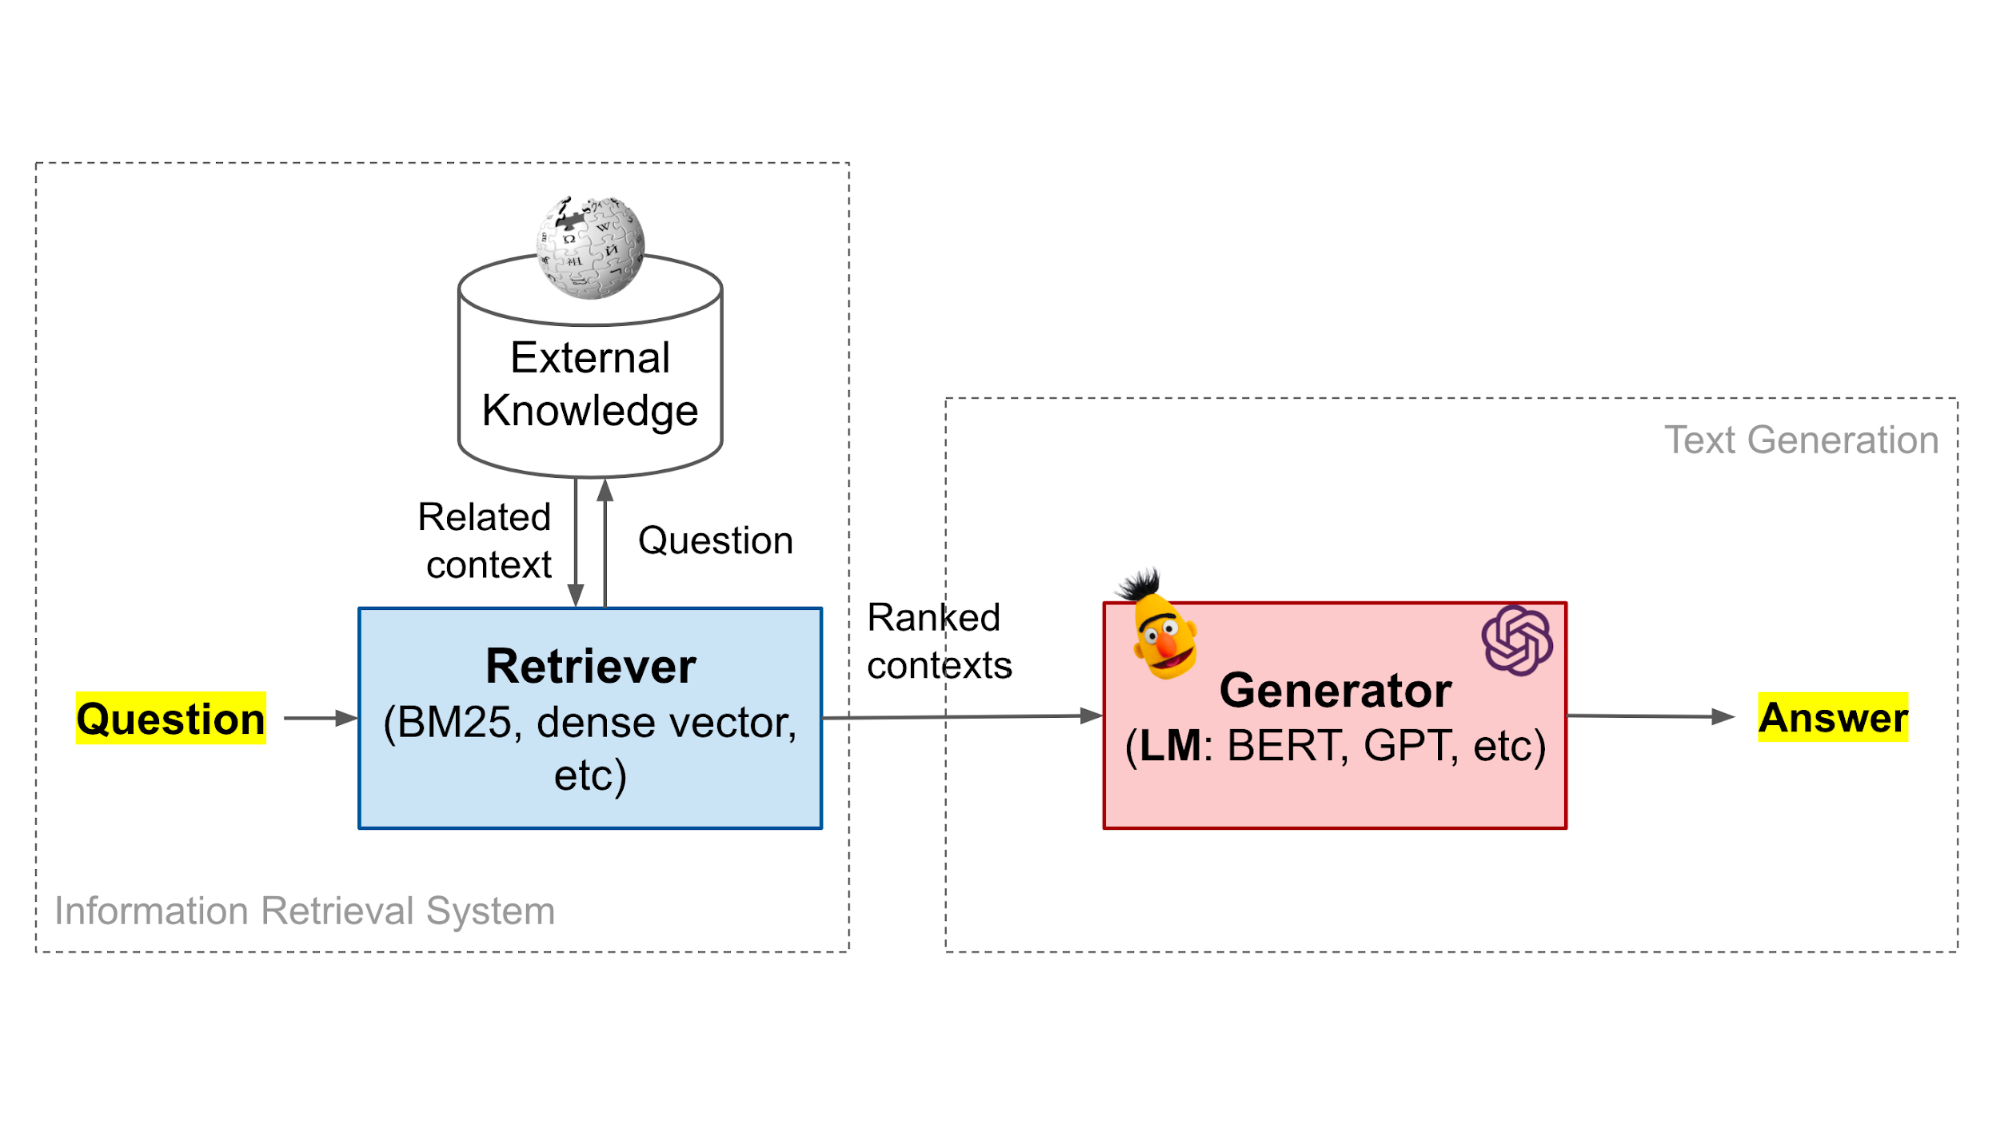
\includegraphics[width=0.82\textwidth]{figures/retrieve-reader-gen.pdf}}
\end{center}
\end{frame}


% \begin{frame}{What RAG Actually Is (and Is Not)}
% % \irStage{DEFINITION}
% \textbf{RAG is a compound AI system, not a single model trick or simple recipe.}

% \vspace{0.8em}
% \begin{itemize}
%   \item \textbf{Not}: just ``BM25 + GPT'' or simple hallucination reduction
%   \item \textbf{Is}: a pipeline of Retrieval + Conditioning + Generation
%   \item \textbf{Core Axes}: retrieval quality, strategy, reasoning, feedback, cost
% \end{itemize}

% \vspace{0.5em}
% \cpause
% \begin{block}{Design Principle}
% \textbf{Modularity} allows isolated debugging.\\
% If generation fails, we must know if it was due to poor retrieval or poor conditioning.
% \end{block}

% \vspace{0.5em}
% \cpause
% \textbf{Key Thesis}
% \begin{itemize}
%   \item \textbf{Retrieval defines the reasoning substrate.}
%   \item If the evidence is not retrieved, it cannot be used by the model.
% \end{itemize}
% \end{frame}

\begin{frame}{A System View: RAG as a Pipeline of Decisions}
% \irStage{SYSTEM ARCHITECTURE}
\textbf{Basic Pipeline: Retrieval, Conditioning, and Generation.}

\vspace{0.5em}
\begin{center}
\resizebox{1.0\textwidth}{!}{
\input{tikz/rag_system_view_simple.tex}
}
\end{center}
\end{frame}



% % ====================================================================
% \section{Part 5 --- The Original RAG Model (Lewis et al.\ 2020)}
% % ====================================================================

% \begin{frame}[plain]
% \sectionpage
% \end{frame}


\begin{frame}{Original RAG Architecture (Lewis et al.\ 2020)}
% \irStage{ARCHITECTURE}
\begin{center}
\fbox{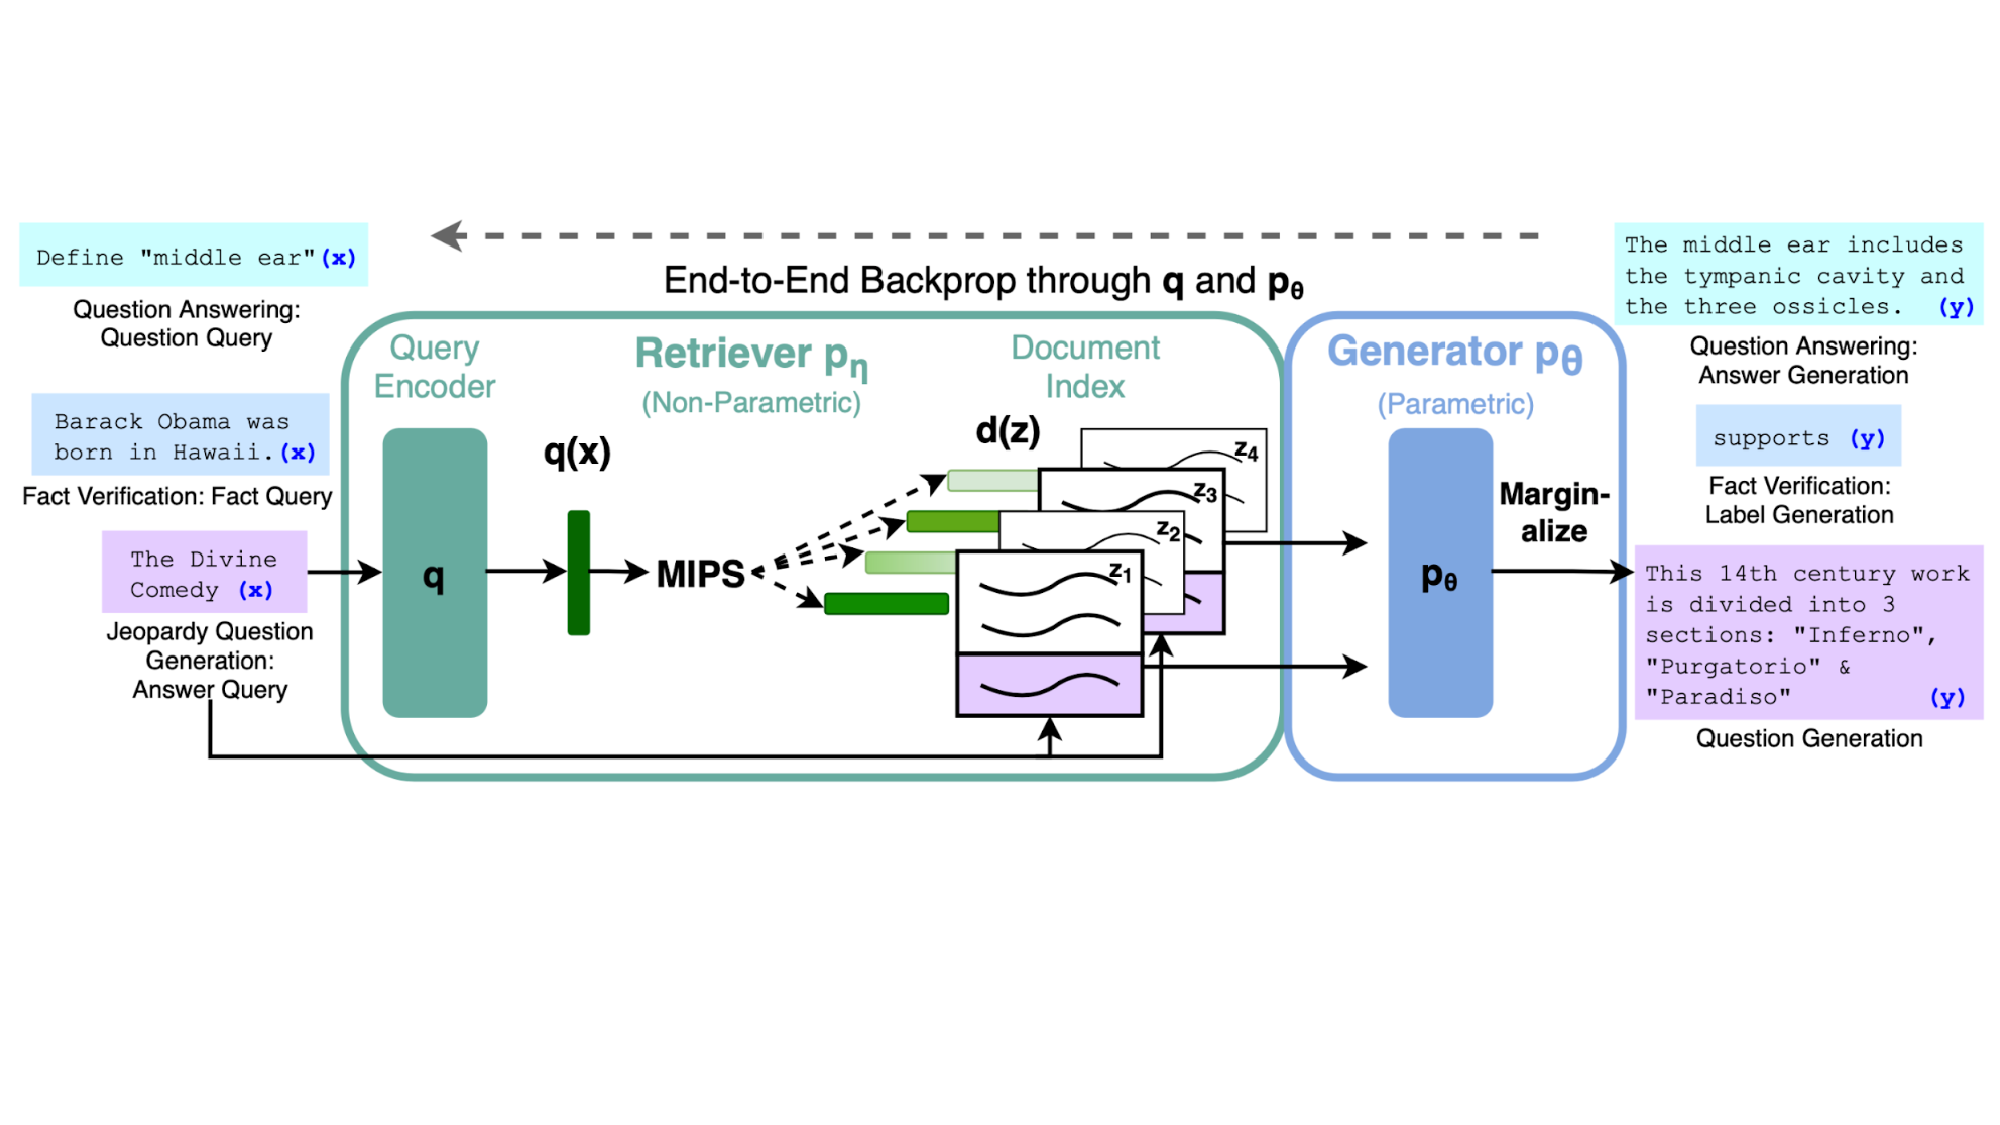
\includegraphics[width=1.0\textwidth]{figures/rag-original.pdf}}
\end{center}
\end{frame}


\begin{frame}[shrink=20]{Lewis et al.\ 2020: The RAG Paper}
% \irStage{FOUNDATIONAL WORK}
\textbf{The paper that named and formalised RAG as a learning framework.}

\vspace{0.7em}
\begin{block}{Two variants}
\begin{itemize}
  \item \textbf{RAG-Sequence}: retrieve once for the full answer
    \[ p(y \mid x) \approx \sum_{z} p(z \mid x)\, p(y \mid x, z) \]
  \item \textbf{RAG-Token}: retrieve per generated token (more flexible, costlier)
\end{itemize}
\end{block}
\cpause
\begin{block}{Components}
\begin{itemize}
  \item \textbf{Non-parametric memory}: Wikipedia DPR FAISS index
  \item \textbf{Parametric memory}: BART-large generator
  \item \textbf{Training}: end-to-end with MIPS-based approximate gradient
\end{itemize}
\end{block}

\cpause
\textbf{Key Innovation}
\begin{itemize}
  \item Retrieval is treated as a \emph{latent variable}.
  \item Marginalising over top-$k$ retrieved documents makes retrieval differentiable in expectation.
\end{itemize}
\end{frame}


\begin{frame}{Sequential Training in RAG}
% \irStage{TRAINING}
\textbf{Retriever and generator can be trained jointly or sequentially.}

\vspace{0.7em}
\begin{enumerate}
  \item \textbf{Stage 1}: Pre-train or fine-tune the dense retriever (DPR, Contriever)
    using in-batch negatives or hard negatives
  \item \textbf{Stage 2}: Joint fine-tuning: marginalise over retrieved passages
    \[ p(a \mid q) = \sum_{z \in \mathcal{R}_k(q)} p(a \mid q, z)\, p(z \mid q) \]
  \item \textbf{Stage 3}: RLHF or DPO for grounding preferences
\end{enumerate}
\end{frame}

\begin{frame}{Sequential Training in RAG: Practical Default}
% \irStage{TRAINING}
\textbf{Joint training is expensive and often unnecessary.}

\vspace{0.7em}
\begin{block}{Practical default (2025)}
\large
Freeze the retriever (Contriever or e5-large).\\[0.5em]
LoRA-fine-tune the generator on grounded QA pairs.
\end{block}
\end{frame}

% ====================================================================
\section{Part 3 --- Retrieval Deep Dive}
% ====================================================================

\begin{frame}[plain]
\sectionpage
\end{frame}

\begin{frame}{What are the retrieval decisions that need to be made?}
% \irStage{SYSTEM ARCHITECTURE}
\begin{center}
\resizebox{1.0\textwidth}{!}{
\input{tikz/rag_system_view_simple_retrieval.tex}
% rag_system_view_simple_query
}
\end{center}
\end{frame}

\begin{frame}{Retrieval Choices in RAG (2025 View)}
% \irStage{RETRIEVAL}
\textbf{Choosing the right retriever involves precision/recall and OOD robustness trade-offs.}

\vspace{0.7em}
\begin{table}
\centering
\resizebox{0.92\textwidth}{!}{
\begin{tabular}{l l l l}
\toprule
\textbf{Method} & \textbf{Strengths} & \textbf{Typical Failure} & \textbf{RAG Default?} \\
\midrule
BM25         & Entity precision, OOD robust, no GPU & Vocabulary mismatch          & Yes (baseline) \\
Dense (DPR)  & Semantic matching, recall             & Entity drift, OOD fragility  & With fine-tuning \\
Hybrid       & Best practical default                & Normalization complexity      & \textbf{Yes} \\
ColBERT      & High quality at scale (late interaction) & Storage, infra cost        & High-value domains \\
\bottomrule
\end{tabular}
}
\end{table}

\cpause
\vspace{0.3em}
\begin{block}{The Ceiling}
\textbf{Retrieval defines the reasoning substrate.}
Most ``hallucinations'' in RAG are \emph{selection failures}: the evidence existed but was not retrieved.
\end{block}
\end{frame}

\begin{frame}{The Evidence Ceiling}
% \irStage{THEORY}
\textbf{A grounded answer is a function of the query and the retrieved evidence.}

\vspace{0.8em}
\[ \text{Answer}(q) = f\!\left(q,\, \mathcal{R}_k(q)\right) \]
\cpause
\begin{itemize}
  \item If $e^\star \notin \mathcal{R}_k(q)$, then $P(\text{correct} \mid q) \approx 0$
  \item \textbf{Retrieve}: find the right chunk
  \item \textbf{Select}: include it in the context window
  \item \textbf{Use}: force grounding via prompt constraints
\end{itemize}
\end{frame}

\begin{frame}{The Evidence Ceiling: Implications and Debugging}
% \irStage{THEORY}
\textbf{Always measure Recall@k \emph{before} tuning the generator.}

\vspace{0.7em}
\begin{block}{Implication}
Improving the generator beyond a certain point yields zero gain if retrieval recall is the bottleneck.
\end{block}

\vspace{0.5em}
\cpause
\begin{block}{Debugging Mantra}
Before blaming the LLM, verify that the correct evidence was actually in the prompt.
\end{block}
\end{frame}

\begin{frame}[shrink=10]{Chunking: A Modeling Decision}
% \irStage{DATA}
\textbf{The retrieval unit $u$ determines recall, precision, and context efficiency.}

\vspace{0.7em}
\begin{columns}[T]
\begin{column}{0.5\textwidth}
\begin{itemize}
  \item \textbf{Fixed-size}: simple; may split sentences or paragraphs mid-thought
  \item \textbf{Semantic}: boundary at paragraph/section; variable length
  \item \textbf{Recursive}: hierarchical split; balances size and coherence
  \item \textbf{Extraction}: tables (linearised), PDFs (layout-aware)
\end{itemize}
\end{column}
\begin{column}{0.47\textwidth}
\begin{center}
\resizebox{0.95\textwidth}{!}{
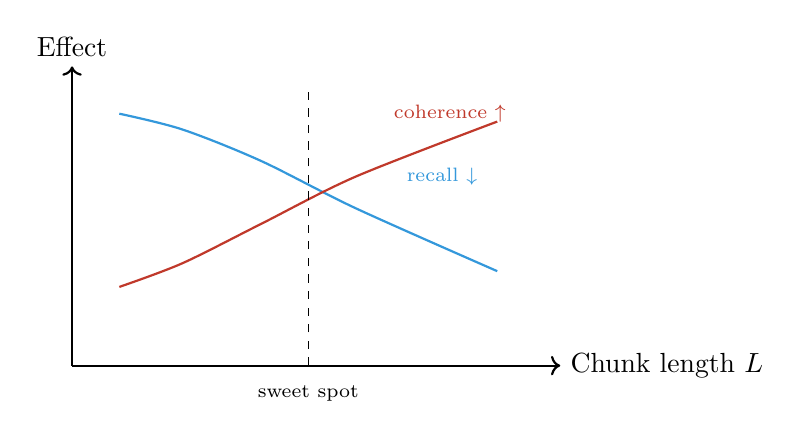
\begin{tikzpicture}[x=1cm,y=1cm]
\draw[->,thick] (0,0) -- (6.2,0) node[right] {Chunk length $L$};
\draw[->,thick] (0,0) -- (0,3.8) node[above] {Effect};
\draw[thick, irSparse] plot[smooth] coordinates {(0.6,3.2) (1.4,3.0) (2.4,2.6) (3.6,2.0) (5.4,1.2)};
\node[irSparse, font=\scriptsize] at (4.7,2.4) {recall $\downarrow$};

\draw[thick, irRerank] plot[smooth] coordinates {(0.6,1.0) (1.4,1.3) (2.4,1.8) (3.6,2.4) (5.4,3.1)};
\node[irRerank, font=\scriptsize] at (4.8,3.2) {coherence $\uparrow$};

\draw[dashed] (3.0,0) -- (3.0,3.5);
\node[font=\scriptsize] at (3.0,-0.35) {sweet spot};
\end{tikzpicture}

}
\end{center}
\end{column}
\end{columns}

\cpause
\vspace{0.4em}
\begin{block}{Rule of Thumb}
Optimise for \textbf{retrievability} and \textbf{citeability}.
A chunk without provenance metadata (doc-id, section, date) breaks the attribution chain.
\end{block}
\end{frame}

\begin{frame}[shrink=20]{Late Chunking: Context-Aware Embeddings}
% \irStage{EMBEDDING}
\textbf{Encode first, pool later---each chunk embedding sees the full document context.}

\vspace{0.5em}
\begin{center}
\resizebox{0.88\textwidth}{!}{
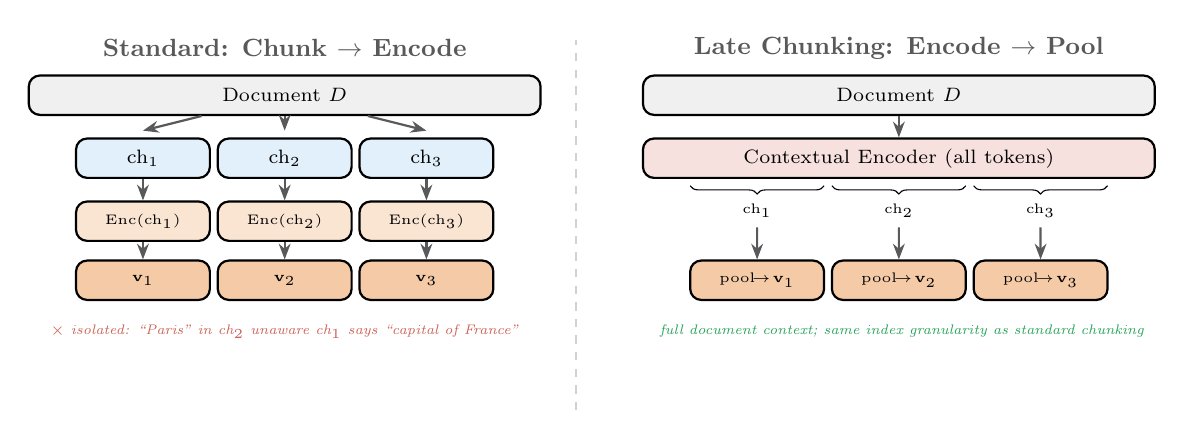
\begin{tikzpicture}[
  box/.style={draw, rounded corners, thick, align=center, font=\scriptsize,
              minimum height=0.5cm},
  arr/.style={-{Stealth[length=2mm]}, thick, draw=irInfra},
  head/.style={font=\small\bfseries, text=irInfra}
]

% Vertical separator
\draw[gray!35, dashed, thick] (0.1, -2.5) -- (0.1, 2.2);

% ===== LEFT: Standard approach =====
\node[head] at (-3.6, 2.1) {Standard: Chunk $\to$ Encode};

\node[box, fill=gray!12, minimum width=6.5cm] (doc1) at (-3.6, 1.5) {Document $D$};

\node[box, fill=irSparse!15, minimum width=1.7cm] (ch1) at (-5.4, 0.7) {ch$_1$};
\node[box, fill=irSparse!15, minimum width=1.7cm] (ch2) at (-3.6, 0.7) {ch$_2$};
\node[box, fill=irSparse!15, minimum width=1.7cm] (ch3) at (-1.8, 0.7) {ch$_3$};

\node[box, fill=irDense!20, minimum width=1.7cm, font=\tiny] (e1) at (-5.4,-0.1) {Enc(ch$_1$)};
\node[box, fill=irDense!20, minimum width=1.7cm, font=\tiny] (e2) at (-3.6,-0.1) {Enc(ch$_2$)};
\node[box, fill=irDense!20, minimum width=1.7cm, font=\tiny] (e3) at (-1.8,-0.1) {Enc(ch$_3$)};

\node[box, fill=irDense!40, minimum width=1.7cm, font=\tiny] (v1) at (-5.4,-0.85) {$\mathbf{v}_1$};
\node[box, fill=irDense!40, minimum width=1.7cm, font=\tiny] (v2) at (-3.6,-0.85) {$\mathbf{v}_2$};
\node[box, fill=irDense!40, minimum width=1.7cm, font=\tiny] (v3) at (-1.8,-0.85) {$\mathbf{v}_3$};

\draw[arr] (doc1) -- (-5.4, 1.05);
\draw[arr] (doc1) -- (-3.6, 1.05);
\draw[arr] (doc1) -- (-1.8, 1.05);
\draw[arr] (ch1)--(e1); \draw[arr] (ch2)--(e2); \draw[arr] (ch3)--(e3);
\draw[arr] (e1)--(v1); \draw[arr] (e2)--(v2); \draw[arr] (e3)--(v3);

\node[font=\tiny\itshape, text=irRerank!80, align=center] at (-3.6,-1.5)
      {$\times$ isolated: ``Paris'' in ch$_2$ unaware ch$_1$ says ``capital of France''};

% ===== RIGHT: Late Chunking =====
\node[head] at (4.2, 2.1) {Late Chunking: Encode $\to$ Pool};

\node[box, fill=gray!12, minimum width=6.5cm] (doc2) at (4.2, 1.5) {Document $D$};
\node[box, fill=irRerank!15, minimum width=6.5cm] (enc) at (4.2, 0.7)
      {Contextual Encoder (all tokens)};

\node[box, fill=irDense!40, minimum width=1.7cm, font=\tiny] (p1) at (2.4,-0.85) {pool$\!\to\!\mathbf{v}_1$};
\node[box, fill=irDense!40, minimum width=1.7cm, font=\tiny] (p2) at (4.2,-0.85) {pool$\!\to\!\mathbf{v}_2$};
\node[box, fill=irDense!40, minimum width=1.7cm, font=\tiny] (p3) at (6.0,-0.85) {pool$\!\to\!\mathbf{v}_3$};

\draw[decorate, decoration={brace, amplitude=3pt, mirror}]
      (1.55, 0.35) -- (3.25, 0.35) node[midway, below=3pt, font=\tiny] (b1) {ch$_1$};
\draw[decorate, decoration={brace, amplitude=3pt, mirror}]
      (3.35, 0.35) -- (5.05, 0.35) node[midway, below=3pt, font=\tiny] (b2) {ch$_2$};
\draw[decorate, decoration={brace, amplitude=3pt, mirror}]
      (5.15, 0.35) -- (6.85, 0.35) node[midway, below=3pt, font=\tiny] (b3) {ch$_3$};

\draw[arr] (doc2) -- (enc);
\draw[arr] (b1) -- (p1); \draw[arr] (b2) -- (p2); \draw[arr] (b3) -- (p3);

\node[font=\tiny\itshape, text=irHybrid!80!black, align=center] at (4.2,-1.5)
      {$\checkmark$ full document context; same index granularity as standard chunking};

\end{tikzpicture}

}
\end{center}

\cpause
\vspace{0.1em}
\begin{block}{Late Chunking (Günther et al., 2024)}
\footnotesize
Encode the full document, then mean-pool the token representations belonging to each chunk.
Same storage footprint as standard chunking; significantly better embedding coherence for long documents.
\end{block}
\end{frame}


\begin{frame}{What are the query modelling decisions that need to be made?}
% \irStage{SYSTEM ARCHITECTURE}
\begin{center}
\resizebox{1.0\textwidth}{!}{
\input{tikz/rag_system_view_simple_query.tex}
% rag_system_view_simple_query
}
\end{center}
\end{frame}

\begin{frame}[shrink=10]{Query Reformulation: Aligning Intent}
% \irStage{RETRIEVAL}
\textbf{Bridging the lexical gap between user questions and document structure.}

\vspace{0.8em}
\begin{block}{Reformulation strategies}
\begin{itemize}
  \item \textbf{HyDE} (Gao et al., 2023): generate a hypothetical document,
    use its embedding as the query vector
  \item \textbf{Multi-query}: generate diverse paraphrases; retrieve for each;
    fuse with RRF
  \item \textbf{Step-back}: abstract the specific question to a broader concept
    before retrieval
  \item \textbf{Decomposition}: break multi-part questions into sub-queries
\end{itemize}
\end{block}

\cpause
\textbf{Intent Drift}
\begin{itemize}
  \item Reformulation can shift user intent.
  \item Always monitor retrieval overlap between original and rewritten queries to detect drift away from the user's actual need.
\end{itemize}
\end{frame}

\begin{frame}[shrink=22]{Retrieval Quality: What to Measure in RAG}
% \irStage{EVALUATION}
\textbf{Standard IR metrics apply---but the grounding question adds a new dimension.}

\vspace{0.7em}
\begin{block}{Standard metrics}
\begin{itemize}
  \item \textbf{Recall@k}: does the gold evidence appear in top-$k$?
  \item \textbf{MRR}: mean reciprocal rank of first relevant passage
  \item \textbf{nDCG@k}: graded relevance; handles multi-answer queries
\end{itemize}
\end{block}
\cpause
\begin{block}{RAG-specific metric}
\textbf{Context Hit Rate}: fraction of queries where the retrieved context contains sufficient information to answer correctly---measured against ground truth answer presence.
\end{block}

\cpause
\vspace{0.3em}
\textbf{Measurement order matters}
\begin{itemize}
  \item Measure Recall@k first. If $< 0.7$, fix the retriever.
  \item Only then tune the generator.
  \item Skipping this is the most common RAG engineering mistake.
\end{itemize}
\end{frame}

% ====================================================================
\section{Part 4 --- Beyond Single-Shot: Multi-Step Retrieval}
% ====================================================================

\begin{frame}[plain]
\sectionpage
\end{frame}

\begin{frame}[shrink=10]{DeRIVeR: Decouple Retrieval and Reasoning}
% \irStage{PARADIGM}
\textbf{Single-shot RAG fails on complex queries that require iterative refinement.}

\vspace{0.7em}
\begin{block}{Single-shot limitation}
$q \to \mathcal{R}_k(q) \to a$\\[0.3em]
One retrieval round captures only the \emph{surface} question. Multi-hop or ambiguous queries require intermediate reasoning steps.
\end{block}

\cpause
\vspace{0.5em}
\begin{block}{DeRIVeR paradigm}
Decouple into three independent roles:
\begin{enumerate}
  \item \textbf{Query Planner}: decompose $q$ into sub-queries
  \item \textbf{Retrieval Module}: execute each sub-query
  \item \textbf{Reasoning Module}: synthesise over accumulated evidence
\end{enumerate}
\end{block}
\end{frame}

\begin{frame}{Strategy 3: Chain-of-Thought Query Decomposition --- Intuition}
% \irStage{QUERY PLANNING}
\begin{block}{Core Idea}
Decompose complex queries into \textbf{atomic sub-queries}, retrieve evidence for each independently, then merge the results. More recall, less vocabulary mismatch.
\end{block}

\vspace{0.8em}
\begin{center}
\resizebox{0.6\textwidth}{!}{
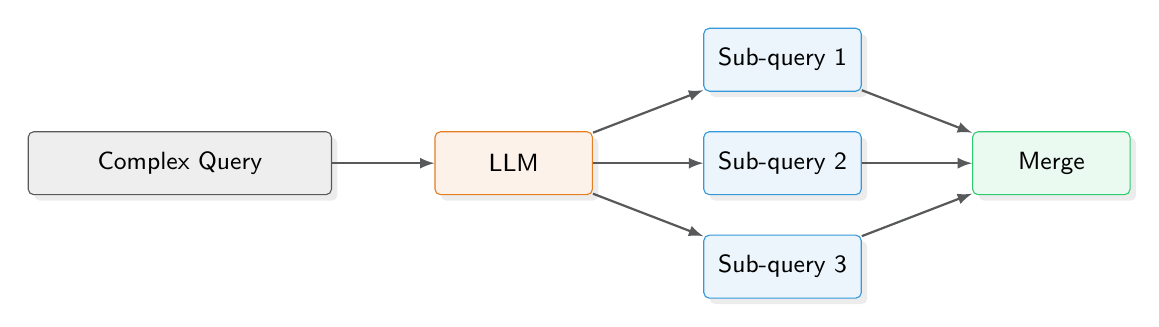
\begin{tikzpicture}[node distance=0.9cm, every node/.style={font=\small\sffamily}]
    \node[infra, text width=3.5cm, align=center] (cq) {Complex Query};
    \node[dense, right=1.3cm of cq] (llm) {LLM};
    \node[sparse, above right=0.5cm and 1.4cm of llm, minimum width=2cm] (sq1) {Sub-query 1};
    \node[sparse, right=1.4cm of llm, minimum width=2cm] (sq2) {Sub-query 2};
    \node[sparse, below right=0.5cm and 1.4cm of llm, minimum width=2cm] (sq3) {Sub-query 3};
    \node[hybrid, right=1.4cm of sq2] (merge) {Merge};
    \draw[irArrowBase] (cq) -- (llm);
    \draw[irArrowBase] (llm) -- (sq1);
    \draw[irArrowBase] (llm) -- (sq2);
    \draw[irArrowBase] (llm) -- (sq3);
    \draw[irArrowBase] (sq1) -- (merge);
    \draw[irArrowBase] (sq2) -- (merge);
    \draw[irArrowBase] (sq3) -- (merge);
\end{tikzpicture}
}
\end{center}
\end{frame}

\begin{frame}[shrink=10]{Query Planning and Decomposition}
% \irStage{QUERY PLANNING}
\textbf{Complex questions require a structured retrieval plan before any search begins.}

\vspace{0.7em}
\begin{block}{Example: sequential decomposition}
\textbf{Q}: ``Who is the CEO of the company that acquired DeepMind, and where did they study?''\\[0.3em]
$q_1$: ``Company that acquired DeepMind'' $\to$ \emph{Google}\\
$q_2$: ``CEO of Google'' $\to$ \emph{Sundar Pichai}\\
$q_3$: ``Education of Sundar Pichai'' $\to$ \emph{IIT Kharagpur, Stanford}
\end{block}

\cpause
\vspace{0.5em}
\begin{block}{Planning strategies}
\begin{itemize}
  \item \textbf{Sequential}: $q_i$ uses result of $q_{i-1}$
  \item \textbf{Parallel}: independent sub-queries; fuse results
  \item \textbf{Conditional}: branch based on intermediate evidence
\end{itemize}
\end{block}
\end{frame}

\begin{frame}[shrink=10]{IR-CoT: Interleaving Retrieval and Chain-of-Thought}
% \irStage{ADVANCED}
\textbf{Trivedi et al.\ (2022): generate one CoT step, then retrieve based on it, repeat.}

\vspace{0.7em}
\begin{block}{Algorithm}
\begin{enumerate}
  \item Generate one chain-of-thought sentence
  \item Use that sentence as the retrieval query
  \item Retrieve passage(s)
  \item Continue generation with accumulated evidence
  \item Terminate when the model outputs the answer
\end{enumerate}
\end{block}

\cpause
\vspace{0.5em}
\begin{exampleblock}{Example (HotpotQA)}
\textbf{Q}: ``Which mountain range contains Piz Bernina?'' \\
\textbf{CoT step 1}: ``Piz Bernina is a peak...'' \\
\textbf{Retrieve}: $\to$ passage: ``The Alps contain Piz Bernina...'' \\
\textbf{CoT step 2}: ``Therefore the Alps.'' $\to$ \textbf{Answer: The Alps}
\end{exampleblock}
\end{frame}

\begin{frame}[shrink=10]{Adaptive RAG: Routing by Complexity}
% \irStage{ADVANCED}
\textbf{Not every query needs the most expensive retrieval strategy.}

\vspace{0.8em}
\begin{center}
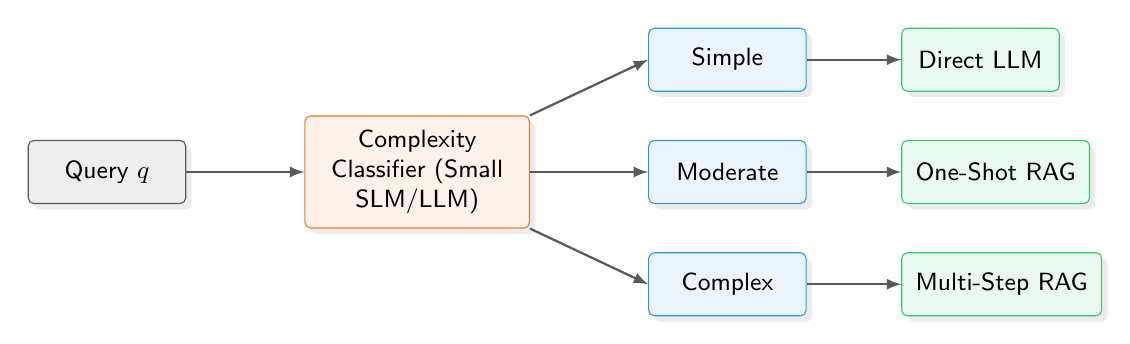
\begin{tikzpicture}[node distance=1.2cm, every node/.style={font=\small\sffamily}]
    \node[infra] (q) {Query $q$};
    \node[dense, right=1.5cm of q, text width=2.5cm, align=center] (router) {Complexity Classifier (Small SLM/LLM)};
    
    \node[sparse, above right=0.3cm and 1.5cm of router] (simple) {Simple};
    \node[sparse, right=1.5cm of router] (moderate) {Moderate};
    \node[sparse, below right=0.3cm and 1.5cm of router] (complex) {Complex};
    
    \node[hybrid, right=1.2cm of simple] (llm) {Direct LLM};
    \node[hybrid, right=1.2cm of moderate] (singleshot) {One-Shot RAG};
    \node[hybrid, right=1.2cm of complex] (multistep) {Multi-Step RAG};
    
    \draw[irArrowBase] (q) -- (router);
    \draw[irArrowBase] (router.north east) -- (simple.west);
    \draw[irArrowBase] (router.east) -- (moderate.west);
    \draw[irArrowBase] (router.south east) -- (complex.west);
    
    \draw[irArrowBase] (simple) -- (llm);
    \draw[irArrowBase] (moderate) -- (singleshot);
    \draw[irArrowBase] (complex) -- (multistep);
\end{tikzpicture}
\end{center}

\cpause
\begin{block}{Key Idea}
Use a classifier to route queries to the most efficient processing path.
Saves latency and tokens for "head" queries while preserving accuracy for the "long tail".
\end{block}
\end{frame}

\begin{frame}{Self-RAG: Selective Retrieval with Critique Tokens}
% \irStage{ADVANCED}
\textbf{Asai et al.\ (2023): train the LM to decide \emph{when} to retrieve and \emph{whether} to trust it.}

\vspace{0.8em}
\begin{block}{Key innovation}
Fine-tune LM to generate \textbf{reflection tokens} alongside regular tokens:
\begin{itemize}
  \item \texttt{[RETRIEVE]}: should I search now?
  \item \texttt{[ISREL]}: is this passage relevant to the question?
  \item \texttt{[ISSUP]}: does the passage support my output?
  \item \texttt{[ISUSE]}: is my overall response useful?
\end{itemize}
\end{block}

\cpause
\vspace{0.5em}
\begin{block}{Benefit}
Not every query needs retrieval.
Self-RAG retrieves only when uncertainty is high---reducing cost and latency.
\end{block}
\end{frame}

\begin{frame}{Self-RAG: Architecture}
% \irStage{ADVANCED}
\begin{center}
\resizebox{0.8\textwidth}{!}{
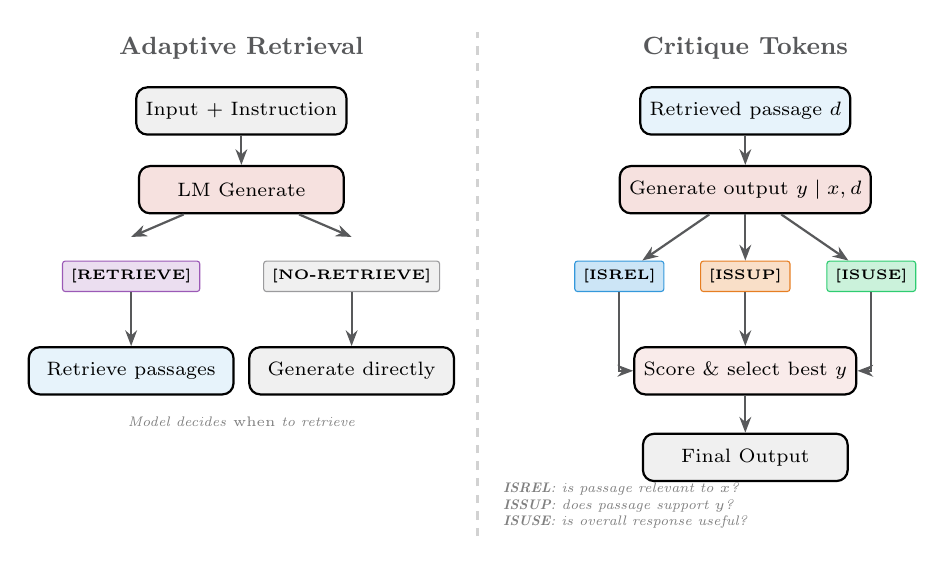
\begin{tikzpicture}[
  box/.style={draw, rounded corners, thick, align=center, font=\scriptsize,
              minimum height=0.6cm, minimum width=2.6cm},
  tok/.style={draw, rounded corners=1pt, font=\tiny\bfseries, inner sep=3pt},
  arr/.style={-{Stealth[length=2mm]}, thick, draw=irInfra},
  lab/.style={font=\tiny\itshape, text=gray}
]

% ===== LEFT: Retrieve-or-not decision =====
\node[font=\small\bfseries, text=irInfra] at (-3.0, 3.4) {Adaptive Retrieval};

\node[box, fill=gray!12] (inp) at (-3.0, 2.6) {Input + Instruction};
\node[box, fill=irRerank!15] (lm)  at (-3.0, 1.6) {LM Generate};

\node[tok, fill=irANN!20, draw=irANN]       (ret)  at (-4.4, 0.5) {[RETRIEVE]};
\node[tok, fill=irMuted!40, draw=irInfra!60] (nret) at (-1.6, 0.5) {[NO-RETRIEVE]};

\node[box, fill=irSparse!12] (retr) at (-4.4, -0.7) {Retrieve passages};
\node[box, fill=gray!12]     (gen2) at (-1.6, -0.7) {Generate directly};

\draw[arr] (inp) -- (lm);
\draw[arr] (lm)  -- (-4.4, 1.0);
\draw[arr] (lm)  -- (-1.6, 1.0);
\draw[arr] (ret)  -- (retr);
\draw[arr] (nret) -- (gen2);

\node[lab] at (-3.0, -1.35)
      {Model decides \emph{when} to retrieve};

% vertical separator
\draw[gray!35, thick, dashed] (0, -2.8) -- (0, 3.6);

% ===== RIGHT: Critique token grading =====
\node[font=\small\bfseries, text=irInfra] at (3.4, 3.4) {Critique Tokens};

\node[box, fill=irSparse!12] (pass) at (3.4, 2.6)
      {Retrieved passage $d$};
\node[box, fill=irRerank!15] (gen3) at (3.4, 1.6)
      {Generate output $y \mid x, d$};

\node[tok, fill=irSparse!25, draw=irSparse] (isrel) at (1.8, 0.5)
      {[ISREL]};
\node[tok, fill=irDense!25, draw=irDense]   (issup) at (3.4, 0.5)
      {[ISSUP]};
\node[tok, fill=irHybrid!25, draw=irHybrid] (isuse) at (5.0, 0.5)
      {[ISUSE]};

\node[box, fill=irRerank!10] (sel)  at (3.4, -0.7) {Score \& select best $y$};
\node[box, fill=gray!12]     (out)  at (3.4, -1.8) {Final Output};

\draw[arr] (pass) -- (gen3);
\draw[arr] (gen3) -- (isrel);
\draw[arr] (gen3) -- (issup);
\draw[arr] (gen3) -- (isuse);
\draw[arr] (isrel) |- (sel);
\draw[arr] (issup) -- (sel);
\draw[arr] (isuse) |- (sel);
\draw[arr] (sel)   -- (out);

% Token legend
\node[lab, align=left, anchor=north west] at (0.2, -2.0) {
  \textbf{ISREL}: is passage relevant to $x$? \\
  \textbf{ISSUP}: does passage support $y$? \\
  \textbf{ISUSE}: is overall response useful?
};

\end{tikzpicture}

}
\end{center}
\end{frame}

% ====================================================================
\section{Part 5 --- Engineering Reality: The LLM Stack}
% ====================================================================

\begin{frame}[plain]
\sectionpage
\end{frame}

\begin{frame}[shrink=12]{The LLM Stack in Practice}
% \irStage{ENGINEERING}
\begin{center}
\fbox{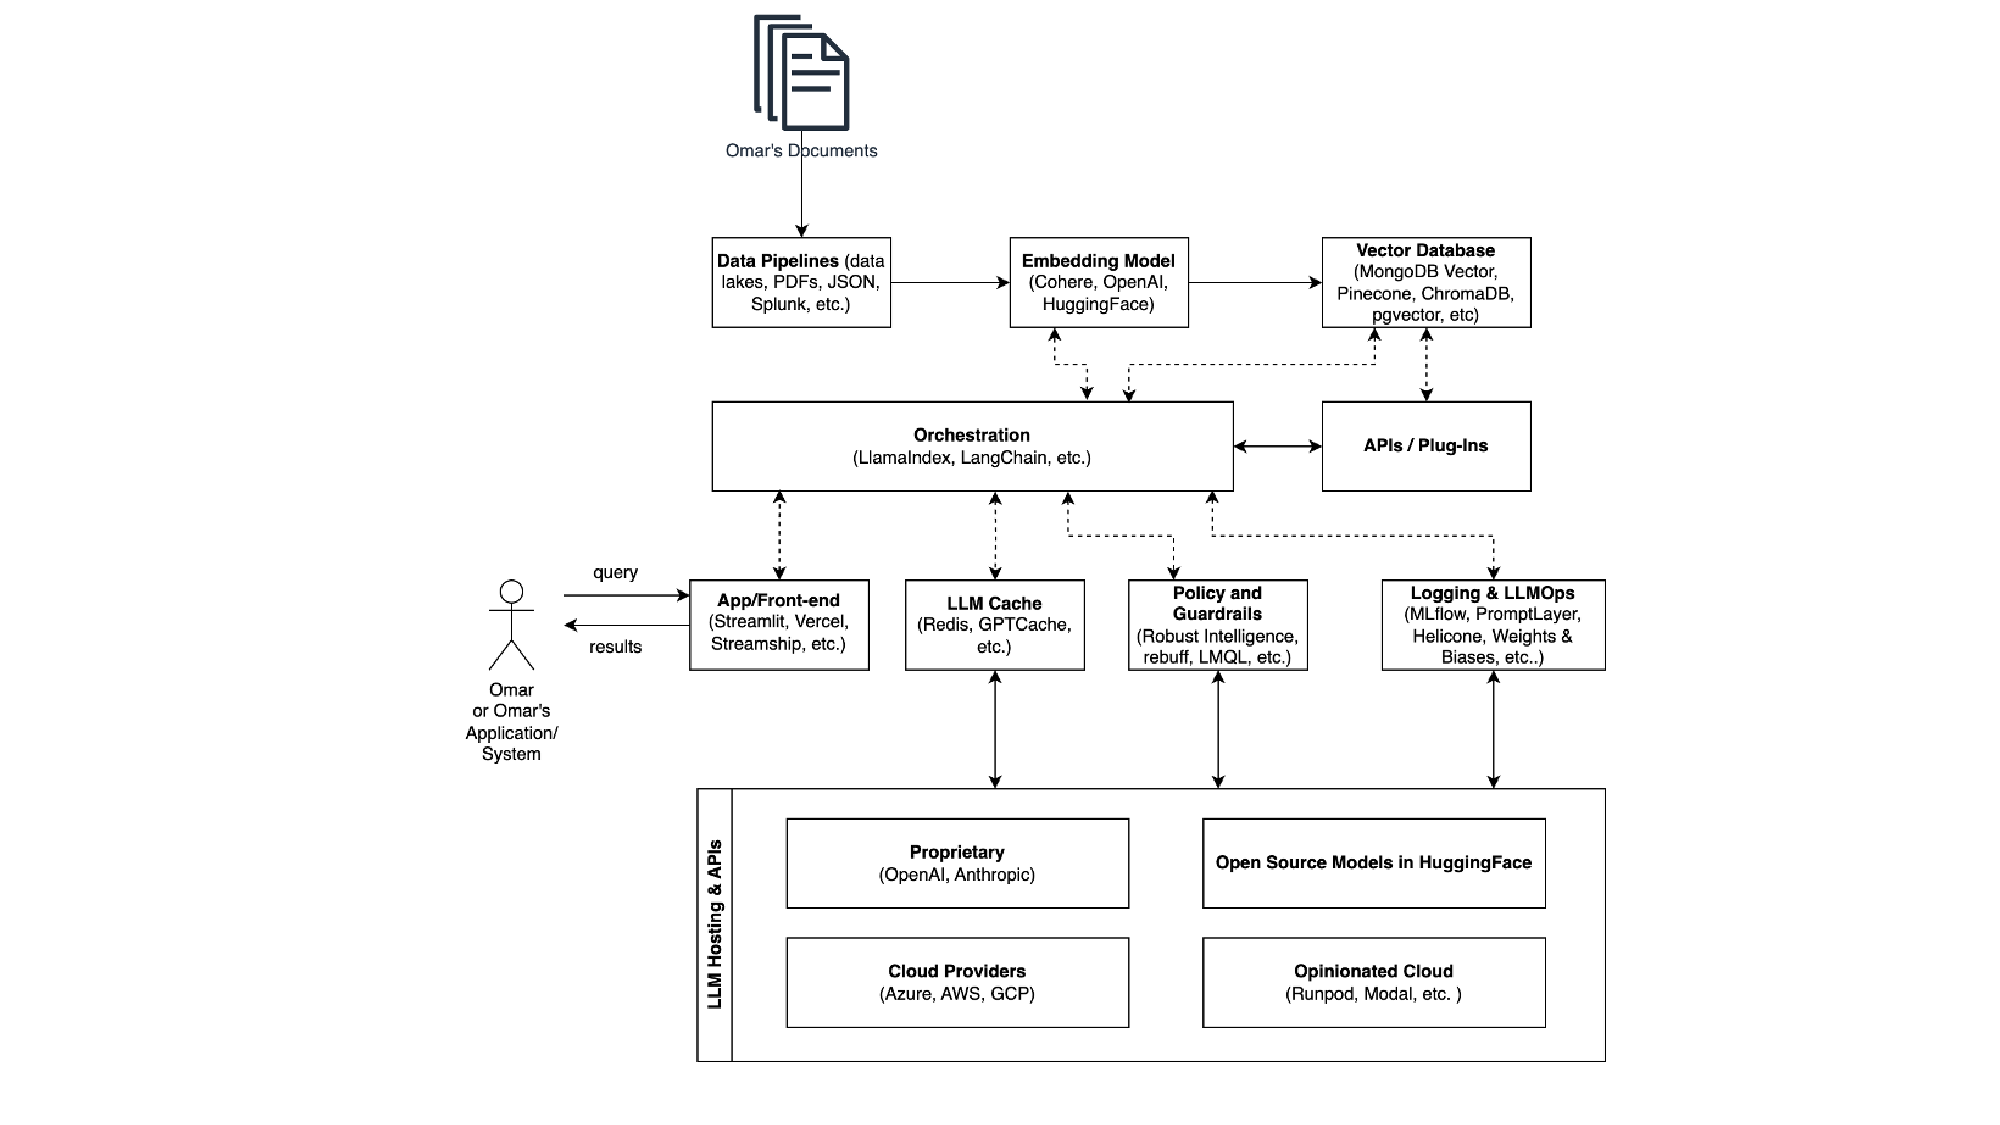
\includegraphics[height=0.75\textheight, keepaspectratio]{figures/llm-stack-cisco.pdf}}
\end{center}
\end{frame}

\begin{frame}[shrink=20]{RAG frameworks}
% \irStage{FRAMEWORKS}
\begin{columns}[T]
\begin{column}{0.48\textwidth}
\begin{center}
\textbf{LlamaIndex}\\[0.5em]
\fbox{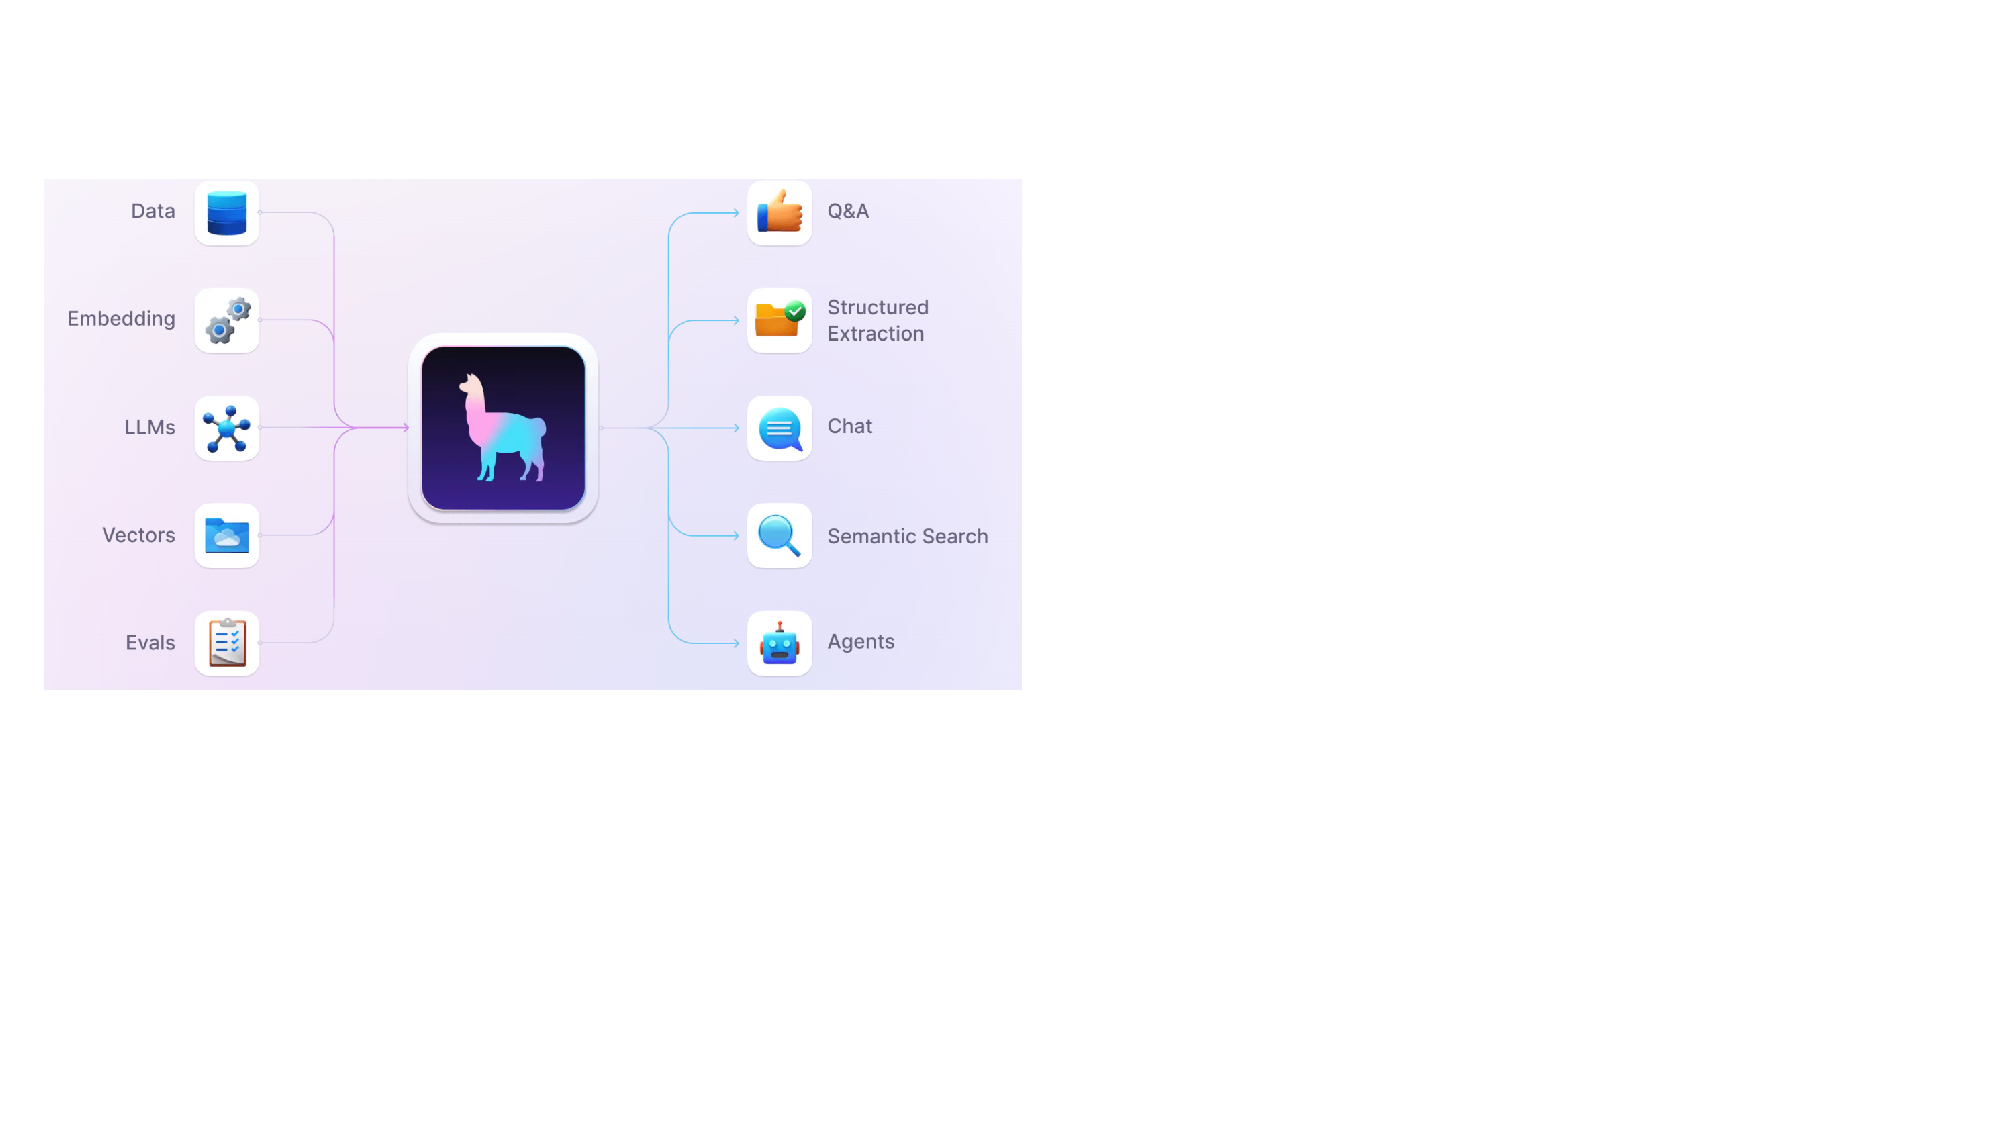
\includegraphics[height=0.45\textheight, keepaspectratio]{figures/llama-index.pdf}}
\end{center}
\end{column}
\begin{column}{0.48\textwidth}
\begin{center}
\textbf{LangChain}\\[0.5em]
\fbox{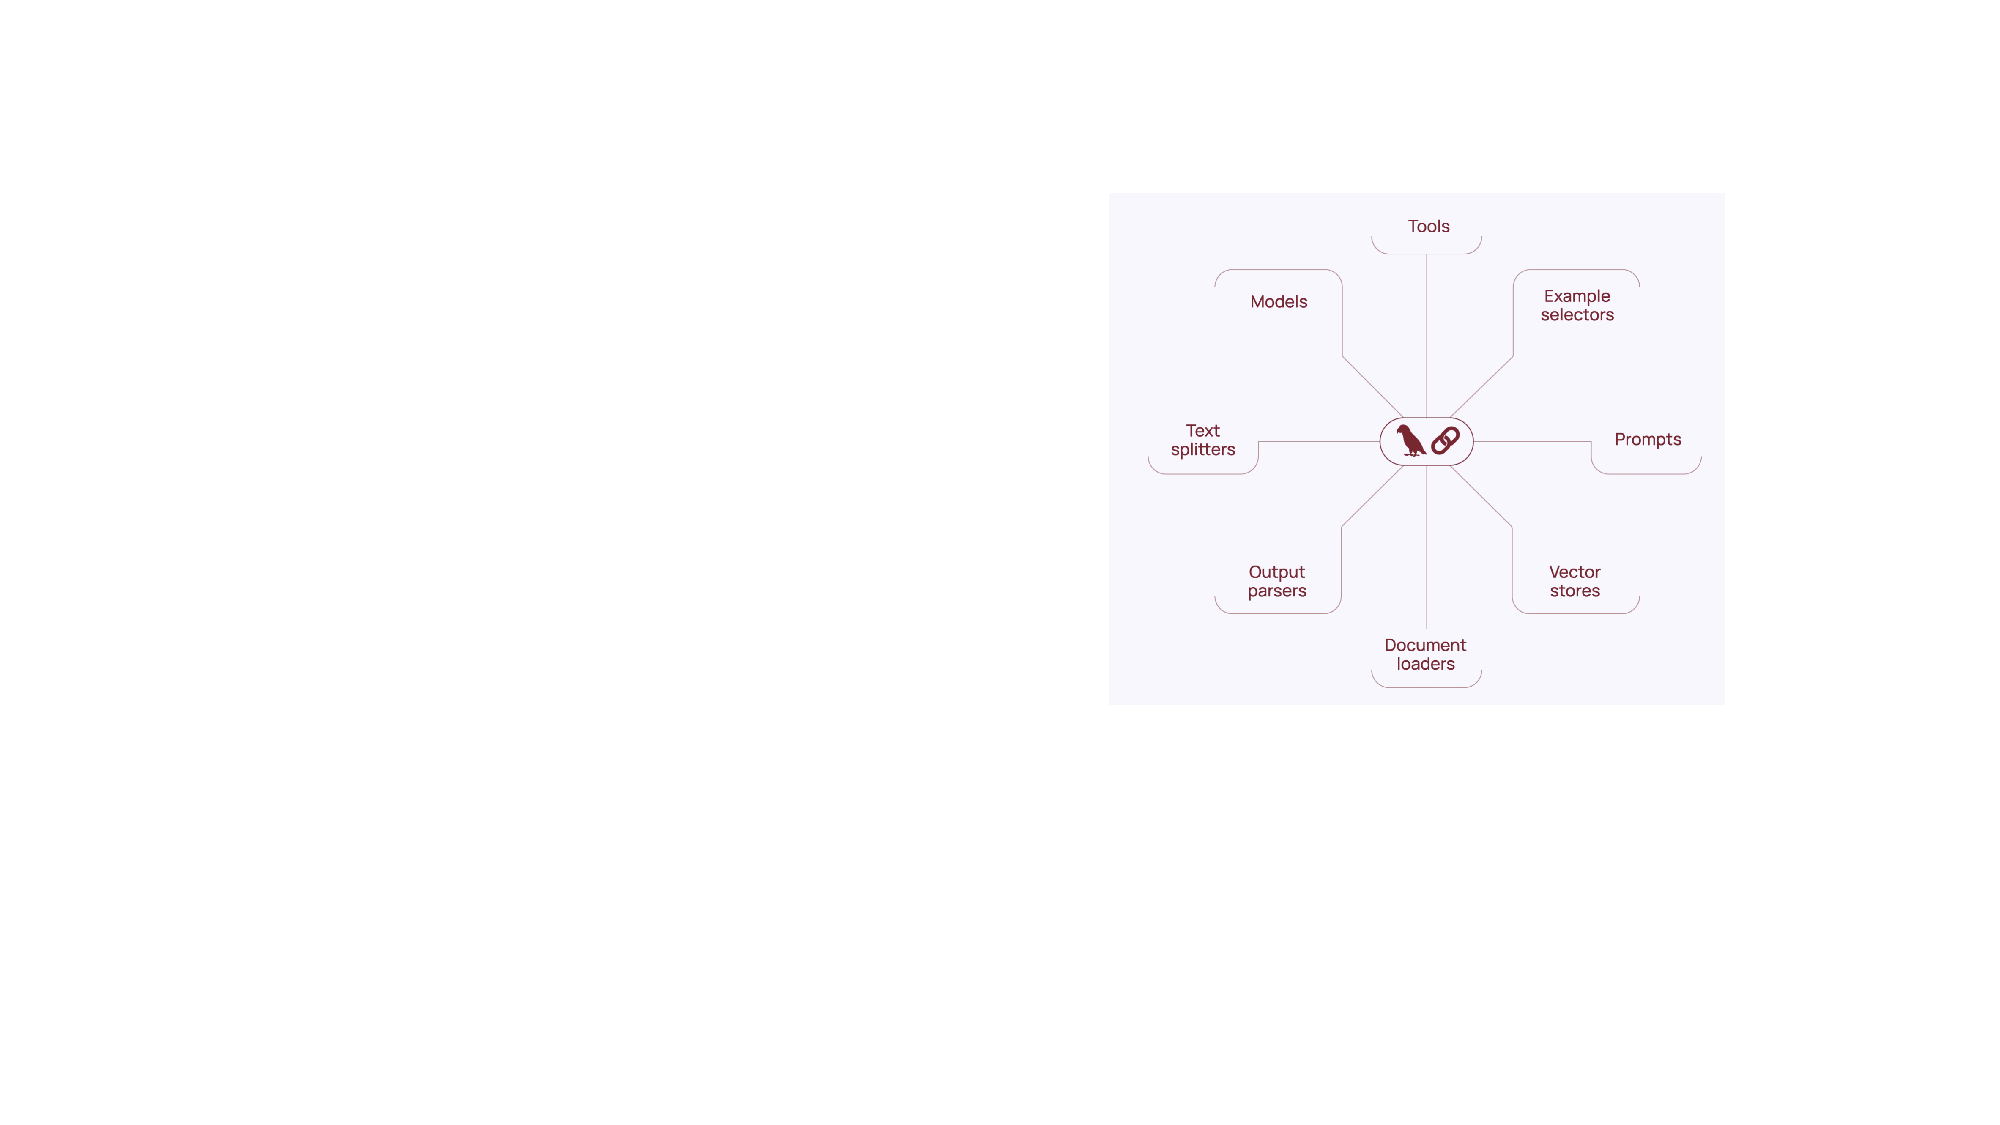
\includegraphics[height=0.45\textheight, keepaspectratio]{figures/langchain.pdf}}
\end{center}
\end{column}
\end{columns}
\end{frame}

\begin{frame}[shrink=20]{What Frameworks Give You (and Don't)}
% \irStage{ENGINEERING}
\textbf{Frameworks accelerate prototyping but do not solve the hard problems.}

\vspace{0.7em}
\begin{columns}[T]
\begin{column}{0.48\textwidth}
\begin{block}{What you get}
\begin{itemize}
  \item Connectors: vector stores, LLM APIs, loaders
  \item Basic retrieval chains (one-shot RAG)
  \item Prompt templates and output parsers
  \item Callback hooks for logging
\end{itemize}
\end{block}
\end{column}
\begin{column}{0.48\textwidth}
\begin{block}{What you don't get}
\begin{itemize}
  \item Retrieval quality evaluation
  \item Production monitoring / drift detection
  \item Cost and latency SLO management
  \item Custom retrieval logic for your domain
\end{itemize}
\end{block}
\end{column}
\end{columns}

\vspace{0.5em}
\cpause
\begin{block}{Lesson}
Use frameworks for the prototype phase.
\textbf{Own your retrieval stack} in production---the framework abstraction will become a ceiling.
\end{block}
\end{frame}


\begin{frame}{A System View: RAG in Production}
% \irStage{SYSTEM ARCHITECTURE}
\textbf{Production deployments require feedback loops and continuous evaluation.}

\vspace{0.5em}
\begin{center}
\resizebox{0.82\textwidth}{!}{
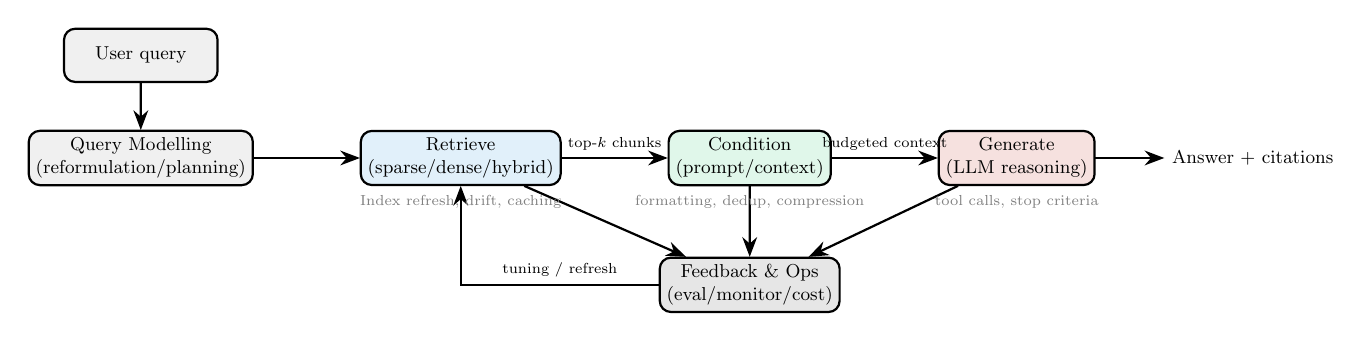
\begin{tikzpicture}[
  scale=0.75, transform shape,
  node distance=1.1cm and 1.2cm,
  box/.style={draw, rounded corners, thick, align=center, minimum height=0.9cm, minimum width=2.6cm, font=\small},
  arr/.style={-{Stealth[length=2.5mm]}, thick}
]
\node[box, fill=gray!12] (query_mod) {Query Modelling\\(reformulation/planning)};
\node[box, fill=gray!12, above=0.8cm of query_mod] (user) {User query};
\node[box, fill=irSparse!15, right=1.8cm of query_mod] (retr) {Retrieve\\(sparse/dense/hybrid)};
\node[box, fill=irHybrid!15, right=1.8cm of retr] (cond) {Condition\\(prompt/context)};
\node[box, fill=irRerank!15, right=1.8cm of cond] (gen) {Generate\\(LLM reasoning)};
\node[box, fill=irInfra!15, below=1.2cm of cond] (fb) {Feedback \& Ops\\(eval/monitor/cost)};

\draw[arr] (user) -- (query_mod);
\draw[arr] (query_mod) -- (retr);
\draw[arr] (retr) -- node[above, font=\scriptsize] {top-$k$ chunks} (cond);
\draw[arr] (cond) -- node[above, font=\scriptsize] {budgeted context} (gen);
\draw[arr] (gen) -- ++(2.5,0) node[right, font=\small] {Answer + citations};

\draw[arr] (gen) -- (fb);
\draw[arr] (retr) -- (fb);
\draw[arr] (cond) -- (fb);
\draw[arr] (fb) -| (retr) node[pos=0.25, font=\scriptsize, above] {tuning / refresh};

\node[font=\scriptsize, text=gray] at ($(retr)+(0,-0.75)$) {Index refresh, drift, caching};
\node[font=\scriptsize, text=gray] at ($(cond)+(0,-0.75)$) {formatting, dedup, compression};
\node[font=\scriptsize, text=gray] at ($(gen)+(0,-0.75)$) {tool calls, stop criteria};
\end{tikzpicture}

}
\end{center}

\cpause
\vspace{0.3em}
\begin{block}{Evaluation contract per module}
\footnotesize
Retrieval: Recall@k \quad\textbar\quad Conditioning: token budget used \quad\textbar\quad Generation: Faithfulness / Attribution
\end{block}
\end{frame}

% ====================================================================
\section{Part 6 --- Evaluation: The RAG Triad}
% ====================================================================

\begin{frame}[plain]
\sectionpage
\end{frame}

\begin{frame}[shrink=10]{RAG Evaluation: Metrics and Grounding}
% \irStage{EVALUATION}
\textbf{Traditional IR metrics (Recall, nDCG) are necessary but insufficient for RAG systems.}

\vspace{0.8em}
\begin{block}{The RAG Triad}
\begin{itemize}
  \item \textbf{Faithfulness}: is the answer supported by retrieved evidence?
  \item \textbf{Groundedness}: no extra claims beyond the evidence
  \item \textbf{Attribution}: do citations point to the correct supporting blocks?
\end{itemize}
\end{block}

\cpause
\begin{block}{The RAG Score}
\[ \text{Score} = w_1 F + w_2 A - w_3 U \]
\tiny $F$: Faithful\quad $A$: Attributed\quad $U$: Unsupported
\end{block}

\cpause
\begin{block}{Tooling}
\footnotesize
RAGAS, TruLens, UpTrain: automated faithfulness scoring using an LLM-as-judge.
\end{block}
\end{frame}

\begin{frame}[shrink=15]{Failure Taxonomy: Stop Being Vague About Errors}
% \irStage{EVALUATION}
\textbf{Design improvements based on specific module-level failure modes.}

\vspace{0.7em}
\begin{columns}[T]
\begin{column}{0.48\textwidth}
\begin{enumerate}
  \item \textbf{Retrieval failure}: $e^\star$ missing from top-$k$
        $\to$ fix retriever (recall, reformulation)
  \item \textbf{Selection failure}: $e^\star$ retrieved but dropped by truncation/dedup
        $\to$ fix context assembly
  \item \textbf{Reasoning failure}: $e^\star$ in context but misused
        $\to$ fix prompt or generator fine-tuning
  \item \textbf{Grounding failure}: fabricated citations or unsupported claims
        $\to$ fix prompt policy and attribution checker
\end{enumerate}
\end{column}
\begin{column}{0.49\textwidth}
\begin{center}
\resizebox{0.95\textwidth}{!}{
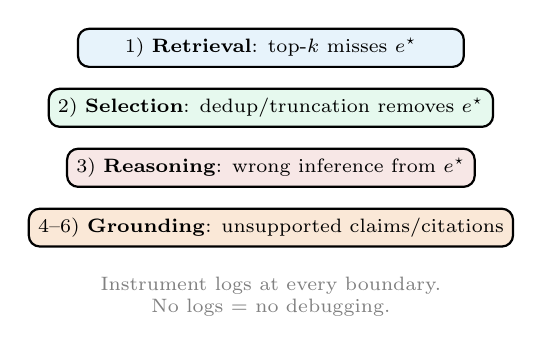
\begin{tikzpicture}[
  box/.style={draw, rounded corners, thick, align=left, font=\scriptsize, minimum width=4.9cm},
  lab/.style={font=\scriptsize, text=gray}
]
\node[box, fill=irSparse!12] (a) {1) \textbf{Retrieval}: top-$k$ misses $e^\star$};
\node[box, fill=irHybrid!12, below=0.25cm of a] (b) {2) \textbf{Selection}: dedup/truncation removes $e^\star$};
\node[box, fill=irRerank!12, below=0.25cm of b] (c) {3) \textbf{Reasoning}: wrong inference from $e^\star$};
\node[box, fill=irDense!18, below=0.25cm of c] (d) {4--6) \textbf{Grounding}: unsupported claims/citations};

\node[lab, below=0.25cm of d, align=center] {Instrument logs at every boundary.\\No logs = no debugging.};
\end{tikzpicture}

}
\end{center}
\begin{block}{}
\footnotesize
Instrument logs at every boundary. No logs = no debugging.
\end{block}
\end{column}
\end{columns}
\end{frame}

% ====================================================================


\begin{frame}{Summary: The 2025 RAG Engineer}
% \irStage{WRAPUP}
\textbf{RAG is a compound system of decisions across data, retrieval, reasoning, and operations.}

\vspace{0.3em}
\begin{block}{Core principles}
\footnotesize
\begin{itemize}
  \item \textbf{Hybrid Default}: always combine Sparse + Dense retrieval
  \item \textbf{Metadata Chains}: preserve provenance from index to prompt
  \item \textbf{Measure First}: Recall@k before tuning the generator
  \item \textbf{Citation Contract}: force claims to cite evidence blocks
  \item \textbf{Evaluation Logs}: retrieve $\to$ select $\to$ prompt $\to$ answer
\end{itemize}
\end{block}

\cpause
\vspace{0.3em}
\begin{block}{Final Takeaway}
\small
If you cannot trace a claim to a retrieved evidence block, you do not have a RAG system.\\[0.5em]
\textbf{Retrieval defines the reasoning substrate.}
\end{block}
\end{frame}

\begin{frame}{Questions?}
\centering
\Large \textbf{Thank you!}

\vspace{2em}
\normalsize
Question Answering and Retrieval-Augmented Generation\\[0.5em]
\small Information Retrieval --- Lecture 7
\end{frame}

\end{document}
